% Author: Jing Li
% License: LaTeX Project Public License v1.3c
% 完整编译: XeLaTex -> BibTex -> XeLaTex -> XeLaTex
% GitHub项目地址:https://github.com/stepbystepcode/agicode

%%%%%%%%%%%%%%%%%%%%%%%%  文档配置  %%%%%%%%%%%%%%%%%%%%%%%%

\documentclass[
    report,     % 文档类型
    oneside,    % 单双栏
    UTF8,       % 字符集
    zihao=-4    % 全局字号(-4是小四号的意思)
]{config} % 配置文件模板 config.cls

% 封面图片定义
\def \titlePageImages{
    
\includegraphics[width=0.48\textwidth] {figures/logos/SXU-logo.pdf}\\ % 山西大学校徽
    \vspace{10pt}
    
\includegraphics[width=0.43\textwidth] {figures/logos/SXU-title.png}\\ % 山西大学校名
}

% 文档信息定义
\def \majorTitle   {软件工程课程论文} % 大标题
\def \minorTitleCN {山西大学课程设计技术报告} % 中文标题
\def \minorTitleEN {Shanxi University Course Design Technical Report} % 英文标题

% 个人信息定义
\def \titlePageInfoBox{
    % 参数:#1下划线长度 #2字号 #3标题 #4内容
    \infobox{8.00cm}{0.65cm}{学生姓名}{李京~赵章词~周培聪~叶隆智}\\
    \infobox{8.00cm}{0.65cm}{专业班级}{计算机科学与技术2202班}\\
    \infobox{8.00cm}{0.65cm}{指导老师}{庞继芳}\\
    \infobox{8.00cm}{0.65cm}{所在院系}{计算机与信息技术学院}\\
}

% 设置行间距为1.5倍
\linespread{1.5}

%%%%%%%%%%%%%%%%%%%%%%%%  文档开始  %%%%%%%%%%%%%%%%%%%%%%%%
\begin{document}

% 封面
\CoverPage
    {right} % 封面类型:both、left、right、empty
    {0.900cm} % 大标题字号大小
    {0.725cm} % 中文标题字号大小
    {0.700cm} % 英文标题字号大小

%%%%%%%%%%%%%%%%%%%%%  正文前页眉页脚  %%%%%%%%%%%%%%%%%%%%%%

% 页眉(关闭页眉务必将页眉类型设为empty)
\Header
    {common} % 页眉类型:common、publish、empty
    {1pt} % 上分隔线宽度
    {1pt} % 两线距离
    {0.5pt} % 下分割线宽度
    {} % 页眉左自定义内容(文本或图片)
    {
\includegraphics[width=0.25\textwidth]{figures/logos/SXU-title-EN.png}} % 页眉中自定义内容(文本或图片)
    {} % 页眉右自定义内容(文本或图片)

%============================================%

% 页脚(关闭页脚务必将页脚类型设为empty) 
\Footer
    {common} % 页脚类型:common、publish、empty
    {0pt} % 上分隔线宽度
    {0pt} % 两线距离
    {0pt} % 下分割线宽度
    {} % 页脚左自定义内容(文本或图片)
    {\thepage} % 页脚中自定义内容(文本或图片)
    {} % 页脚右自定义内容(文本或图片)

%============================================%

% 页数样式 参数:#1起始页数
\SetRomanPageNumber{} % 设置罗马数字页码
% \SetArabicPageNumber{} % 设置阿拉伯数字页码
\ResetCounter{1} % 重置页数

%%%%%%%%%%%%%%%%%%%%%%%%  摘要  %%%%%%%%%%%%%%%%%%%%%%%

\begin{abstractCN}[0.6cm] % 中文摘要,参数:#1中文摘要标题字号

本项目旨在开发基于检索增强生成(RAG)技术的AI编程代理模型,通过精确的文档解析与代码生成优化,提升代码质量和开发者的编程体验。该系统集成了智能文档检索、自动化代码生成与优化,并结合大语言模型(LLM)进行推理处理,能够显著减少开发者在编程过程中的冗余工作。系统设计采用前后端分离架构,前端使用React和TypeScript,后端使用FastAPI与PostgreSQL,AI层利用SGLang Server并结合LangChain技术实现RAG处理。


% 中文关键词
\def\keywordsCN{AI编程代理;RAG;代码生成;文档解析;LangChain;SGLang}

\end{abstractCN}

%============================================%

\begin{abstractEN}[0.6cm] % 英文摘要,参数:#1英文摘要标题字号

This project aims to develop an AI programming assistant model based on Retrieval-Augmented Generation (RAG) technology, enhancing code quality and the programming experience through accurate document parsing and code generation optimization. The system integrates intelligent document retrieval, automated code generation, and optimization, leveraging large language models (LLM) for inference. The design follows a frontend-backend separation architecture, with React and TypeScript on the frontend, FastAPI and PostgreSQL on the backend, and AI inference through SGLang Server and LangChain for RAG processing.

% 英文关键词
\def\keywordsEN{AI Programming Assistant; RAG; Code Generation; Document Parsing; LangChain; SGLang}

\end{abstractEN}

%%%%%%%%%%%%%%%%%%%%%%%%  启用目录  %%%%%%%%%%%%%%%%%%%%%%%%

% 目录,参数: 
% #1目录类型:next(分页显示)、current(同页显示)
% #2目录行距
% #3目录标题
% #4当前章节名
\contentPage{next}{1.5}{目~~~~录}{目录}
% \contentpageOfFigures{next}{1.5}{图目录}{图目录}
% \contentpageOfTables{current}{1.5}{表目录}{表目录}

%%%%%%%%%%%%%%%%%%%%%%%%  启用水印  %%%%%%%%%%%%%%%%%%%%%%%%

% 若正文不需要水印把这部分命令删掉就好
\imageWatermark % 图片水印
    {0} % 旋转角度
    {0.7} % 放缩倍率
    {0.02} % 透明度 0-1
    {figures/logos/SXU-logo.eps} % 图片路径

%%%%%%%%%%%%%%%%%%%%%%  正文页眉页脚  %%%%%%%%%%%%%%%%%%%%%%%

% 页眉(关闭页眉务必将页眉类型设为empty)
\Header
    {common} % 页眉类型:common、publish、empty
    {1pt} % 上分隔线宽度
    {1pt} % 两线距离
    {0.5pt} % 下分割线宽度
    {Shanxi University} % 页眉左自定义内容(文本或图片)
    {} % 页眉中自定义内容(文本或图片)}
    {\currentChapterInfo} % 页眉右自定义内容(文本或图片)

%============================================%

% 页脚(关闭页脚务必将页脚类型设为empty) 
\Footer
    {common} % 页脚类型:common、publish、empty
    {0pt} % 上分隔线宽度
    {0pt} % 两线距离
    {0pt} % 下分割线宽度
    {} % 页脚左自定义内容(文本或图片)
    {\thepage} % 页脚中自定义内容(文本或图片)
    {} % 页脚右自定义内容(文本或图片)

%============================================%

% 页数样式 参数:#1起始页数
% \SetRomanPageNumber{} % 设置罗马数字页码
\SetArabicPageNumber{} % 设置阿拉伯数字页码
\ResetCounter{1} % 重置页数

%%%%%%%%%%%%%%%%%%%%%%%%%  正文  %%%%%%%%%%%%%%%%%%%%%%%%%%

\chapter{问题定义报告}

\section{项目名称}
码途 CodeWay:基于 RAG 的智能编程辅助系统
\section{背景}
在当今科技飞速发展的时代,人工智能(AI)技术凭借在自然语言处理(NLP)和大模型(LLM)领域的卓越成果,在代码生成、优化及调试等编程环节彰显出巨大潜力,为软件开发流程注入了新的活力。然而,当前市面上广泛应用的通用 AI 编程助手,尽管功能强大,却难以规避一些关键弊端。其中,幻觉(Hallucination)现象时有发生,导致生成的代码出现不符合实际逻辑或需求的内容;信息检索方面的不准确,使得开发者获取的参考资料无法切实解决编程难题;更为突出的是,代码质量呈现出参差不齐的状态,在实际项目应用中难以达到理想的稳定性与可靠性标准。
深入探究传统 AI 代码生成模式,其高度依赖现有的大模型。但不容忽视的是,这类模型普遍欠缺精准的外部知识检索能力,这一短板在技术更迭频繁、文档更新迅速的领域,如日新月异的前端框架以及不断升级的后端 API 等场景下,暴露得淋漓尽致。在此情况下,模型极易生成与最新技术规范脱节、存在错误的代码,严重影响了开发者的工作效率与项目质量。
为有效攻克这些难题,显著提升代码生成的准确性与可用性,引入检索增强生成(RAG, Retrieval-Augmented Generation)技术成为极具前景的解决方案。基于对行业现状与技术痛点的深刻洞察,本项目志在构建一个基于 RAG 的 AI 编程代理模型。通过对技术文档进行精确解析,并针对代码生成流程展开全方位优化,致力于最大程度减少幻觉现象,稳步提升代码质量,最终为广大开发者缔造更为优质、高效的使用体验,推动编程领域迈向新的发展阶段。

\section{项目资源}
\begin{itemize}
    \item 操作系统:macOS Sequoia 15.3.2, Ubuntu 22.04
    \item 数据库:Supabase (Self-Hosting, PostgreSQL 15.1)、框架:granian+FastAPI
    \item 前端:React, TypeScript, Tauri2, Shadcn/UI
    \item 后端:Python 3.13, FastAPI, SGLang
    \item CPU: Intel Xeon Platinum 8468V (192) @ 2.401GHz
    \item GPU: NVIDIA H100 80G * 2
    \item RAM: 1TB
\end{itemize}

\section{项目目标}
本项目旨在构建 “码途 CodeWay:基于 RAG 的智能编程辅助系统”,凭借先进的检索增强生成(RAG)技术,彻底革新编程辅助体验。
首要目标是打造精准的代码生成体系。借助 RAG 技术,系统能够深入检索海量的前沿技术文档与代码库,针对开发者输入的编程需求,生成契合最新技术规范且准确无误的代码片段。无论是复杂的算法实现,还是常见的功能模块构建,均可高效输出高质量代码,杜绝因知识滞后导致的错误代码生成。
系统将为开发者提供智能化的代码优化建议。针对既有代码,利用 RAG 技术结合多维度代码质量评估标准,精准定位代码中可优化的部分,如性能瓶颈、代码冗余、安全隐患等,并依据丰富的行业最佳实践案例,给出详尽且切实可行的优化方案,助力开发者提升代码整体质量与运行效率。
同时,强化代码调试支持。在开发者调试过程中,系统通过 RAG 技术迅速匹配相似的调试场景与解决方案,精准定位代码错误根源,提供详细的错误解释以及修复指引,大幅缩短调试时间,提升开发效率。
在个性化服务层面,系统能够学习并适应用户的编程习惯与偏好。依据开发者过往的代码风格、常用技术栈以及解决问题的方式,为其定制个性化的代码生成与优化策略,打造专属于每位开发者的编程辅助环境。
总体而言,“码途 CodeWay” 项目致力于构建一个功能完备、智能高效的编程辅助系统,凭借 RAG 技术解决传统编程辅助工具的痛点,全面提升开发者的编程效率与代码质量,推动软件开发行业迈向智能化、高效化发展新阶段。

% \section{问题概述}
% 在当前AI编程助手的应用过程中,主要存在以下问题:
% \begin{itemize}
%     \item 代码幻觉问题:AI模型在生成代码时,常常会生成错误、不完整或过时的代码,导致开发者需要额外进行修正和调试。
%     \item 信息检索精准度不足:当前的AI代码助手通常无法精准检索目标技术文档,导致生成的代码与最新标准或API不匹配。
%     \item 代码生成的可执行性较低:部分AI生成的代码无法直接运行,需要开发者额外修改,增加了开发成本。
%     \item 难以联动不同文档信息:开发者在查询某个框架或库的API时,可能需要结合多个文档网站的信息,而现有的AI助手难以有效整合不同来源的数据。
%     \item 缺乏代码优化和修复能力:AI生成的代码可能包含性能问题或安全漏洞,但目前的AI工具大多只能提供静态代码建议,而无法智能优化和修复代码。
% \end{itemize}


\section{项目规模}
项目成本约为 20 元,开发周期约 3 个月。

\section{初步设想}
基本功能
\begin{enumerate}[itemsep=2pt,topsep=0.6pt,parsep=0.6pt]
\item 文档 URL 精确检索功能:用户输入相关编程问题或关键词,系统能依据用户提供的文档 URL,在指定文档范围内进行精准检索,快速定位到包含解决方案或相关知识点的内容段落,并将其呈现给用户,辅助用户解决编程疑惑。
\item 代码试运行功能:用户可在系统内输入代码片段,选择目标编程语言及运行环境,点击试运行按钮后,系统迅速执行代码,并将运行结果、控制台输出以及可能出现的错误信息实时反馈给用户,帮助用户快速验证代码逻辑是否正确。
\item 代码纠错机制:当代码试运行出现错误时,系统自动启动纠错机制。利用内置算法和知识库,分析错误类型与代码上下文,为用户提供详细的错误解释、可能的修正建议以及相关参考文档链接,引导用户高效修复代码错误。
\item 模型切换功能:用户可根据自身需求和使用场景,在系统界面便捷切换内置的多个模型,如 ChatGPT4o、Qwen/QwQ32b 等。同时,支持用户自主调用 Hugging Face 平台上的其他模型,满足不同用户对模型性能、风格和专业性的多样化需求。
\item 登录注册功能:用户通过手机号或邮箱进行注册,设置密码后完成账号创建。登录系统后,用户可享受个性化服务,系统将记录用户使用偏好、历史操作记录等信息,为用户提供更贴合需求的编程辅助体验。
\end{enumerate}
用户所具功能
\begin{enumerate}[itemsep=2pt,topsep=0.6pt,parsep=0.6pt]
\item 个人信息管理:用户可在个人中心查看、修改个人注册信息,包括昵称、头像、密码等,设置个性化偏好,如默认编程语言、常用模型选择等。
\item 代码编辑与调试:在系统提供的代码编辑器中输入、编辑代码,利用代码试运行和纠错机制进行代码调试工作。同时,可将常用代码片段收藏,方便后续复用。
\item 模型使用与切换:自由选择系统内置的 ChatGPT 4o、Qwen/QwQ32b 模型,或按照自身需求配置并调用 Hugging Face 平台上的其他模型,享受不同模型带来的差异化编程辅助服务。
\item 文档检索与知识学习:借助文档 URL 精确检索功能,查询特定技术文档获取编程知识。查看系统推荐的相关编程教程、文章链接,提升自身编程技能。
\item 反馈提交:在使用过程中,若遇到问题或有改进建议,可通过反馈渠道向管理员提交,与平台保持互动,助力系统持续优化。
\end{enumerate}
\section{可行性研究}
进行一周,费用不超过 100 元。


\chapter{可行性研究报告}
\section{引言}
\subsection{编写目的}
在当今编程领域,开发者对高效、智能编程辅助工具的需求与日俱增。传统编程辅助手段难以满足开发者在面对复杂项目、快速迭代技术时的迫切需求,亟需一款创新型编程辅助系统。“码途 CodeWay:基于 RAG 的智能编程辅助系统” 应运而生,其致力于凭借前沿的检索增强生成(RAG)技术,实现精准的代码生成、高效的代码优化以及智能的代码调试辅助。
本可行性研究报告旨在全面评估 “码途 CodeWay” 系统的开发价值与实施可行性。通过深入的市场调研,精准把握开发者在编程过程中的痛点与期望,明确系统应具备的核心功能与特性,如精准的文档 URL 检索,助力开发者快速获取有效知识;强大的代码试运行与纠错机制,保障代码的正确性与可靠性;灵活的多模型切换功能,满足不同场景下的编程需求。
从技术视角出发,深入探究当前技术水平能否充分支撑系统各项功能的稳定实现。评估 RAG 技术在实际应用中的成熟度,以及与多模型集成的适配性;考量服务器运载能力是否足以应对大规模用户并发访问,确保系统在高负载下仍能保持高效、稳定运行。在经济层面,详细核算项目开发所需的人力、物力、财力等各项成本,同时结合市场规模、潜在用户群体以及竞争态势,科学预估系统投入使用后的预期收益,确保项目具备良好的投资回报率。此外,严格审视项目在开发与运营过程中是否完全契合现行社会制度及法律法规,杜绝任何潜在的法律风险。
为了在项目开发前对此系统项目进行良好的分析,判断此系统方案是否可实行,而编写此项研究报告。分析应用当前技术以及服务器运载是否可实现,经济预算开支以及预期收益,是否符合社会制度及法律法规。

\subsection{背景}
在数字化浪潮席卷全球的当下,软件开发行业蓬勃发展,编程作为推动科技进步的核心力量,其重要性愈发凸显。随着开源项目的爆发式增长、新技术框架的频繁迭代,编程领域的知识体量呈指数级扩张。与此同时,开发者面临的项目复杂度不断攀升,对编程效率和代码质量的要求也日益严苛。
近年来,人工智能(AI)技术,特别是自然语言处理(NLP)与大模型(LLM)的迅猛发展,为编程辅助领域带来了新的曙光。众多 AI 编程助手纷纷涌现,试图帮助开发者缓解编程压力。然而,当前通用 AI 编程助手暴露出诸多亟待解决的问题。幻觉(Hallucination)现象时有发生,导致生成的代码逻辑混乱、无法运行;信息检索准确性欠佳,使得开发者难以获取精准有效的参考资料;代码质量参差不齐,在实际项目应用中稳定性与可靠性不足。尤其在前端框架、后端 API 等技术文档更新瞬息万变的领域,传统 AI 代码生成模式因过度依赖既有大模型,缺乏精准的外部知识检索能力,极易生成过时或错误代码,严重阻碍了开发进程,降低了开发效率。
在此背景下,检索增强生成(RAG, Retrieval-Augmented Generation)技术崭露头角,为解决上述难题提供了新的思路与方法。RAG 技术能够有效整合外部知识源,实现对最新技术文档的精准检索,并将检索结果融入代码生成过程,从而大幅提升代码生成的准确性与可用性。
“码途 CodeWay:基于 RAG 的智能编程辅助系统” 项目顺势而生。其旨在凭借 RAG 技术的强大优势,构建一个集精准代码生成、高效代码优化、智能代码调试以及个性化编程服务于一体的综合性编程辅助平台。该系统将打破传统编程辅助工具的局限,重塑编程开发流程,为开发者提供更加智能、高效、可靠的编程体验,推动软件开发行业朝着智能化、高效化方向实现跨越式发展,在日新月异的编程技术变革浪潮中,开辟出一条全新的 “码途” 。
\begin{enumerate}[label=(\arabic*)]
    \item 软件系统的名称:码途 CodeWay - 基于 RAG 的智能编程辅助系统
    \item 任务提出者:山西大学
    \item 开发者:李京、赵章词、周培聪、叶隆智
    \item 普通用户:程序员
    \item 实现该软件的计算中心或计算机网络:山西大学计算机与信息技术学院
    \item 该软件系统同其他系统或其他机构的基本的相互来往关系:由山西大学计算机与信息技术学院作为技术支持
\end{enumerate}
\subsection{定义}
\begin{itemize}[itemsep=2pt,topsep=0.6pt,parsep=0.6pt]
    \item React:用于构建用户界面的 JavaScript 库,广泛应用于前端开发,通过组件化的方式来构建复杂的 Web 应用程序。
    \item TypeScript:是 JavaScript 的超集,为 JavaScript 添加了类型系统,使代码更易于维护和扩展,常与 React 等框架一起使用。
    \item Vite:一个快速的前端构建工具,旨在提供更快速的开发体验,尤其适用于现代前端框架,如 React、Vue 等。
    \item Tailwind CSS:是一个高度可定制的 CSS 框架,用于快速构建现代响应式 Web 界面,可与 React 等前端框架无缝集成。
    \item Shadcn/UI:是一个基于 React 和 Tailwind CSS 的 UI 组件库,提供了一系列可复用的高质量 UI 组件,帮助开发者快速搭建美观的用户界面。
    \item FastAPI:基于 Python 的快速 Web 框架,使用类型提示来提高代码的可读性和可维护性,用于构建高性能的后端 API。
    \item PostgreSQL:一种强大的开源关系型数据库管理系统,常用于后端开发中存储和管理数据。
    \item Supabase:一个开源的后端即服务平台,提供了包括数据库(基于 PostgreSQL)、身份验证、存储等一系列功能,方便后端开发。
    \item SGLang:一个针对大型语言模型和视觉语言模型的快速服务框架。它通过共同设计后端运行时和前端语言,让您与模型的交互更快、更可控。
    \item PyTorch:一个广泛使用的开源机器学习库,主要用于深度学习任务,提供了丰富的工具和函数来构建和训练神经网络。
    \item Hugging Face:一个在自然语言处理领域非常知名的平台,提供了大量的预训练模型、工具和数据集,方便开发者进行各种自然语言处理任务,如文本生成、问答系统等。
    \item LangChain:一个用于开发基于语言模型的应用程序的框架,它提供了一系列工具和组件,帮助开发者更轻松地构建和部署与语言模型相关的应用,例如聊天机器人、智能文档处理等。
    \item VectorDB:向量数据库,专门用于存储和管理向量数据,常用于人工智能领域,特别是与机器学习模型结合,用于存储和查询嵌入向量等数据。
    \item Bun:一个快速的 JavaScript 运行时,类似于 Node.js,旨在提供更好的性能和开发体验,可用于前端和后端开发。
    \item Docker:一种容器化技术,用于将应用程序及其依赖项打包成容器,实现环境的隔离和可移植性,方便应用的部署和管理。
    \item Granian:一个基于 Rust 的高性能 Python ASGI 服务器,用于提高 Python Web 应用的性能和并发处理能力。
    \item UV(Python 环境管理器):用于管理 Python 虚拟环境的工具,帮助开发者创建、管理和切换不同的 Python 环境,确保项目依赖的隔离和正确安装。
    \item Tauri:一个构建跨平台桌面应用的框架,使用 Web 技术(HTML、CSS、JavaScript)和 Rust 编写,可将 Web 应用打包成桌面应用。
\end{itemize}
\subsection{参考资料}


\section{可行性研究的前提}
\subsection{要求}
\begin{enumerate}[label=(\arabic*)]
    \item AI编程代理功能
    \begin{enumerate}[label=(\alph*)]
        \item 检索并解析技术文档,提高代码准确性
        \item 生成符合最新标准的代码,并可自动优化
        \item 提供代码错误分析和纠错建议
    \end{enumerate}
    \item 用户所具功能
    \begin{enumerate}[label=(\alph*)]
        \item 查询并获取代码建议
        \item 提交问题并获取最佳代码解决方案
        \item 结合具体开发场景,获取最优代码优化策略
        \item 反馈代码质量,优化AI的生成能力
    \end{enumerate}
    \item 输出要求:数据完整、准确。
    \item 系统功能模块图
    \begin{figure}[h] % 创建一个图片环境,[h]表示图片尽量放在当前位置
    \centering % 使图片居中
    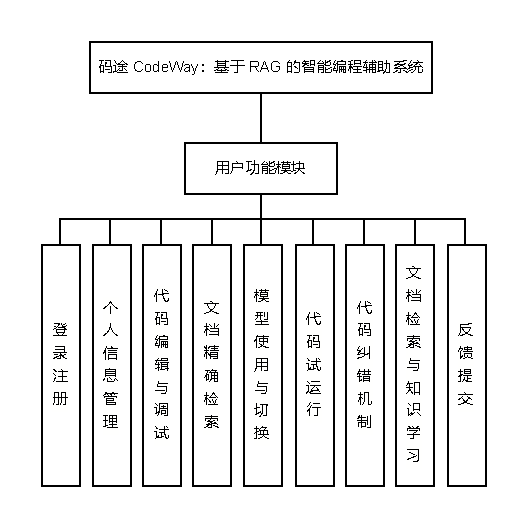
\includegraphics[width=0.8\textwidth]{figures/system-module.pdf}
    \caption{系统功能模块图} % 添加图片标题
    \label{fig:system-module} % 为图片添加标签,方便在文档中引用
\end{figure}
    \item 安全与保密方面的要求:数据库的安全性首先通过视图机制,不同的用户只能访问系统授权的视图,这在一定程度上提高数据库的安全性。系统平台的安全性则体现在操作系统的安全性、计算机系统的安全性和网络体系的安全性等方面。
    \item 同本系统相连接的其他系统:无。
    \item 完成期限:三个月。
\end{enumerate}

\subsection{目标}
\begin{enumerate}[label=(\arabic*)]
    \item 将用户置于决策的核心地位,允许他们自主调整代码生成策略,优化代码推荐体验。本系统作为智能代理,精准解析用户需求,提高代码生成的准确性和可用性。
    \item 引入智能代码优化和错误检测功能,减少开发者在调试和修改过程中的时间成本,提升代码质量。
    \item 通过智能检索算法和数据分析,确保代码生成基于最新的技术文档和行业标准,提升代码的可执行性和稳定性。
    \item 使该平台成为开发者、研究人员和技术团队的重要工具,提供代码管理、文档检索和最佳实践推荐功能,提升开发效率和技术创新能力。
\end{enumerate}

\subsection{条件、假设和限制}
\begin{enumerate}[label=(\arabic*)]
    \item 所建议系统的运行寿命的最小值:5 年
    \item 进行系统方案选择比较的时间:1 个月
    \item 经费来源:项目组自费
    \item 法律和政策方面的限制:无
    \item 硬件环境:CPU core i5 及以上、内存 16G 及以上
    \item 运行环境:Linux 6.10 及以上
    \item 开发环境:MacOS、Ubuntu、VScode、Pycharm
    \item 系统投入使用的最晚时间:2025 年 6 月 15 日
\end{enumerate}

\subsection{进行可行性研究的方法}
本次可行性研究主要运用调查研究法与对比分析法相结合的方式。在调查研究方面,由专业的技术团队与行业专家共同针对广大开发者群体展开调研。通过线上问卷、线下访谈等形式,广泛收集开发者在日常编程工作中遇到的痛点,对现有编程辅助工具的使用体验、功能需求以及期望改进方向等信息。同时,深入各大软件企业、开源社区,了解不同规模项目的编程流程与实际需求,掌握行业内对智能编程辅助系统的应用现状与潜在需求。

在对比分析环节,对市面上现有的主流编程辅助工具,包括但不限于具有代码生成、代码优化功能的工具进行全面剖析。从功能特性、性能表现(如代码生成速度、纠错准确性)、用户口碑、收费模式等多个维度进行详细对比。针对不同类型的编程语言、开发场景下这些工具的适用性展开深入研究,同时密切关注国内外新兴的、具有创新性的编程辅助技术与系统案例,分析其技术原理、优势以及可借鉴之处。

通过此次可行性研究,致力于打造一个契合开发者实际需求、功能完备且性能卓越的“码途CodeWay:基于RAG的智能编程辅助系统”。系统旨在提供精准的代码生成、高效的代码优化建议、智能的代码调试支持,以及个性化的编程服务,帮助开发者显著提升编程效率,降低开发成本,最终为项目的顺利推进与成功落地提供坚实的数据支撑与方向指引。 

\subsection{评价尺度}
\begin{enumerate}[label=(\arabic*)]
    \item 开发费用:100 元
    \item 开发时间:3 个月
    \item 使用中的难易程度:设计从简(适合于任何水平的人员使用)。
\end{enumerate}
\newpage
\section{对现有系统的分析}
\subsection{现有系统分析}
\begin{enumerate}[label=(\arabic*)]
    \item ChatGPT
ChatGPT 是 OpenAI 于 2022 年 11 月 30 日发布的聊天机器人模型,基于 GPT-3.5 和 GPT-4 大模型构建,能以对话方式与用户交互。它在语言表达和生成方面优势显著,回复自然流畅,适合日常闲聊,在创意写作如生成诗歌、故事等内容时表现突出。还具备强大的语言理解能力,可处理各类自然语言文本,理解其中含义与潜在意图,能根据用户输入生成逻辑清晰、语法正确的长文本回复,涵盖代码输出、文字翻译、论文及小说撰写等功能。其插件丰富,进一步拓展了应用场景。不过,它存在 “幻觉” 问题,会生成错误或虚构信息,知识更新也不及时,且缺乏个性化定制。
\begin{figure}[h] % 创建一个图片环境,[h]表示图片尽量放在当前位置
    \centering % 使图片居中
    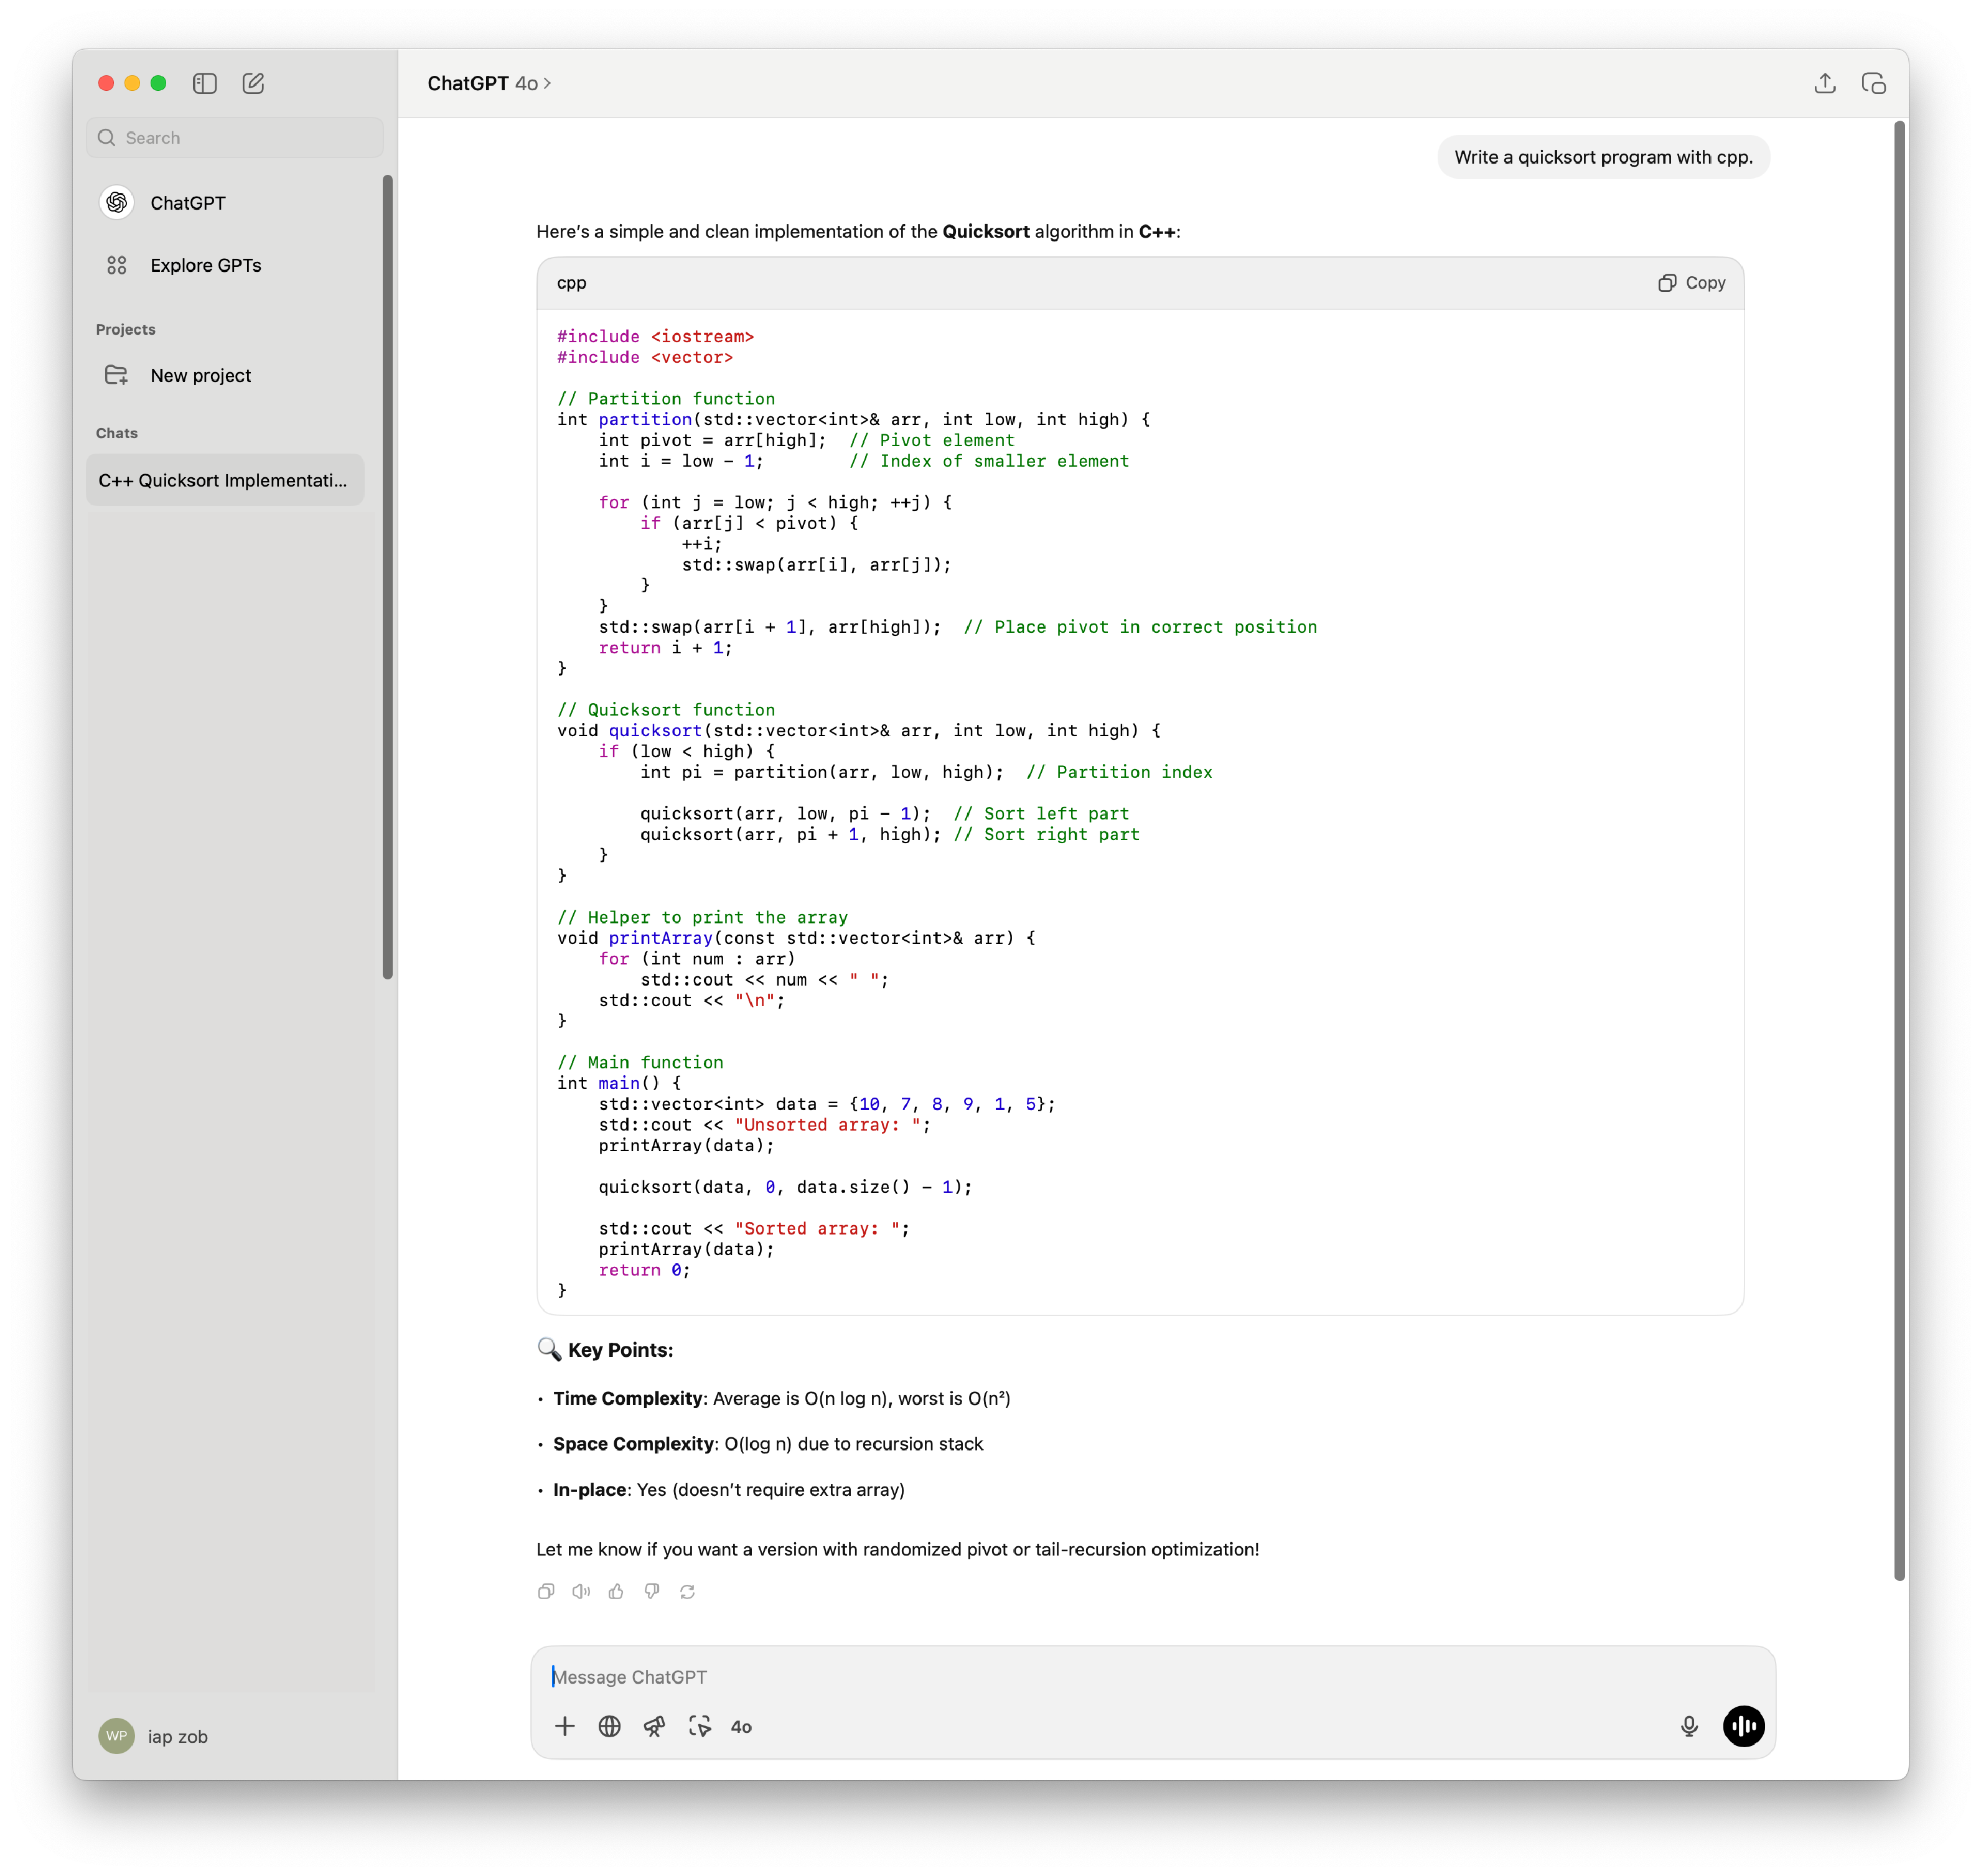
\includegraphics[width=0.8\textwidth]{figures/chatgpt.pdf}
    \caption{ChatGPT界面} % 添加图片标题
    \label{fig:ChatGPT} % 为图片添加标签,方便在文档中引用
\end{figure}
    \item Claude
Claude 是 Anthropic 公司开发的大型语言模型,以强大的自然语言处理能力、卓越的上下文理解能力和高度安全性受关注。知识储备深入,回复准确性高,能全面准确理解用户语言,提供精确回复,还可提供个性化定制服务。采用 “宪法式 AI” 训练方法,减少有害或不当内容生成。在处理长文本方面表现出色,支持 20 万级别的 Token,甚至能处理超 100 万 Token 输入。但相比 ChatGPT,其在某些场景下的多样性受限,市场认知度和应用范围也相对较窄。
\begin{figure}[h] % 创建一个图片环境,[h]表示图片尽量放在当前位置
    \centering % 使图片居中
    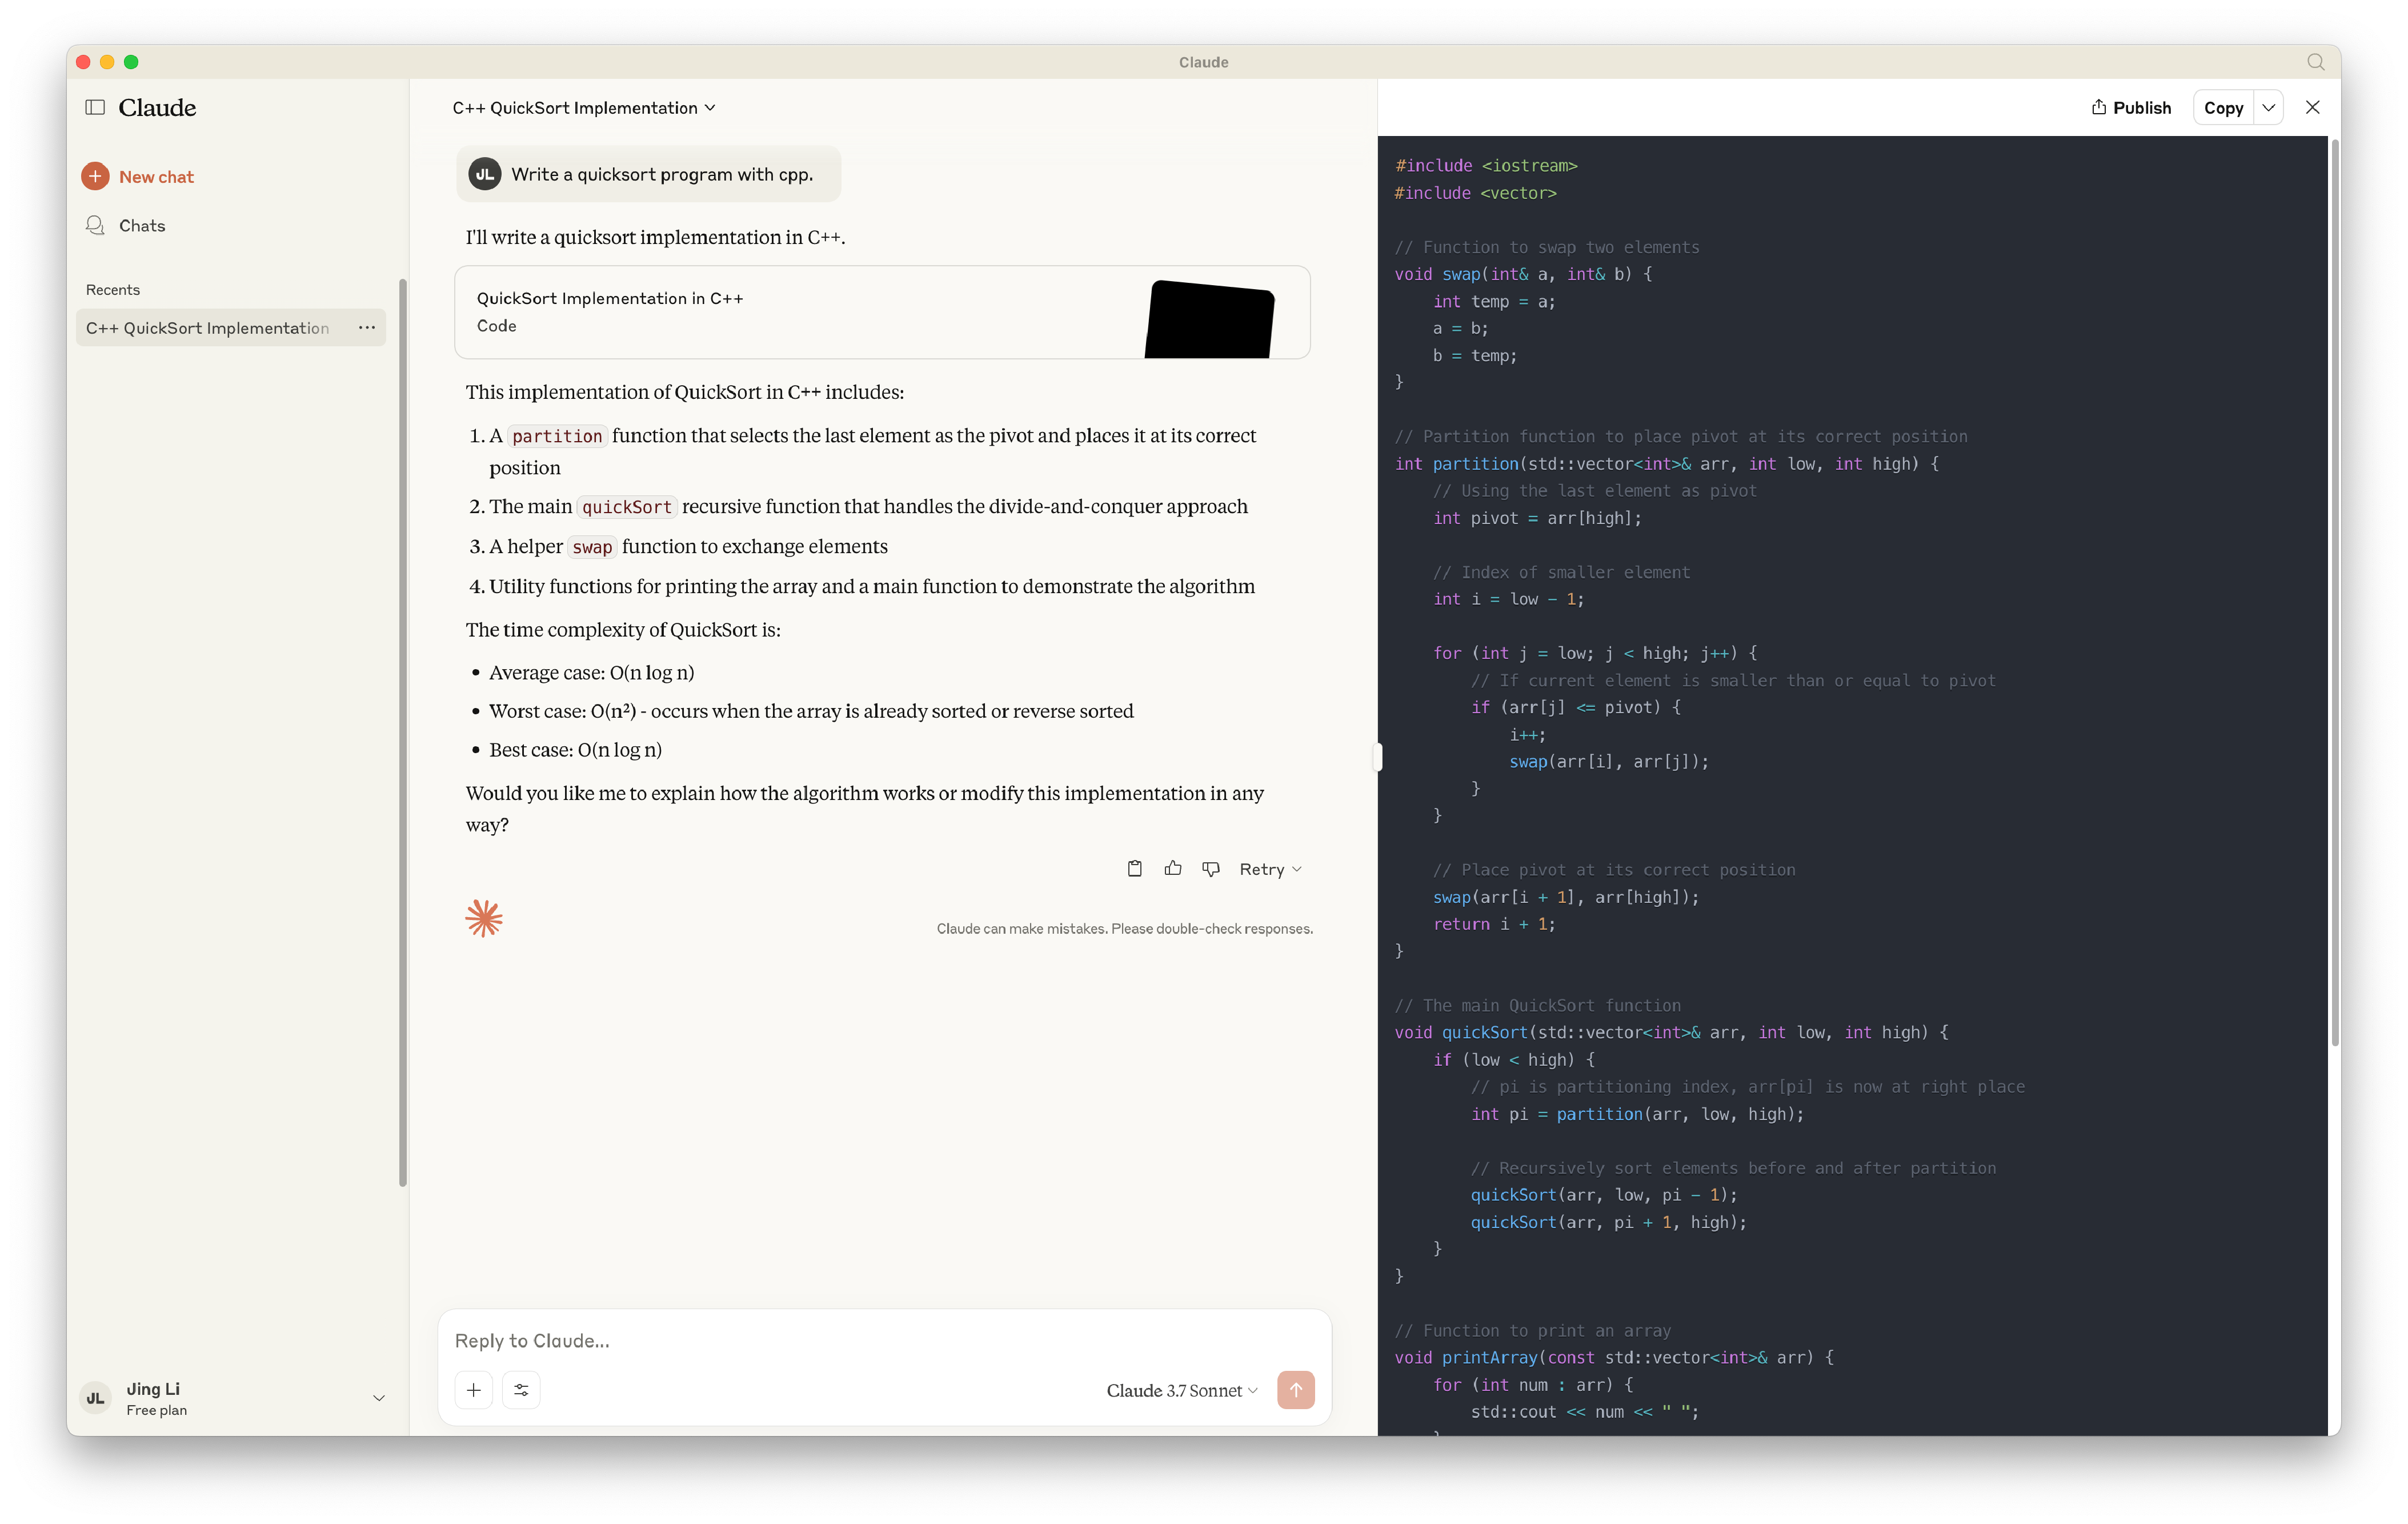
\includegraphics[width=0.8\textwidth]{figures/claude.pdf}
    \caption{Claude界面} % 添加图片标题
    \label{fig:Claude} % 为图片添加标签,方便在文档中引用
\end{figure}
\end{enumerate}
\subsection{新旧系统对比}
\begin{enumerate}[label=(\arabic*)]
    \item 代码生成精准度更高
传统编程辅助系统在代码生成时,常因知识检索不精准或模型自身局限,产生代码错误、过时或不适用的情况。码途 CodeWay 系统借助 RAG 技术,精准检索最新技术文档,生成贴合当下需求且准确无误的代码,极大提升代码生成的质量与可用性。
    \item 代码优化更智能
以往编程辅助工具对代码优化建议较为笼统,缺乏针对性。码途 CodeWay 能依据代码特点,结合行业最佳实践,为开发者提供详细且个性化的代码优化策略,助力开发者高效提升代码性能与质量。
    \item 调试支持更高效
面对代码调试难题,旧系统往往难以快速定位问题根源,提供的解决方案也不尽人意。码途 CodeWay 利用智能算法和海量案例库,迅速分析错误,给出清晰的错误解释及修复指引,大幅缩短调试时长,提高开发效率。
    \item 模型适配灵活性更好
传统系统多依赖单一模型,难以满足开发者多样需求。码途 CodeWay 允许用户自由切换内置的 ChatGPT4o、Qwen/QwQ32b 等模型,还支持调用 Hugging Face 平台其他模型,适配不同开发场景与偏好。
    \item 知识获取更便捷
过去开发者获取编程知识,需在众多文档、论坛中自行筛选。码途 CodeWay 的文档 URL 精确检索功能,可依用户需求,在指定文档内精准定位知识内容,为开发者节省大量查找时间。
    \item 个性化服务更完善
旧系统服务千篇一律,无法满足开发者个性化需求。码途 CodeWay 能学习开发者编程习惯,从代码风格到常用技术栈,提供定制化编程辅助,打造专属编程环境。
\end{enumerate}
\subsection{总结}
码途 CodeWay 系统在设计与应用方面具有显著创新点,同时也面临一系列难点。
创新点体现于多维度。在功能层面,凭借 RAG 技术实现精准代码生成、智能代码优化及高效调试支持,这是传统编程辅助系统难以企及的。例如,能依据最新技术文档生成契合需求的代码,为开发者提供详细且个性化的优化策略。在用户体验上,可自由切换多模型并支持外部模型调用,还能根据用户编程习惯提供定制化服务,极大提升使用的灵活性与便捷性。在知识获取途径上,其文档 URL 精确检索功能,帮助开发者在海量文档中快速定位所需知识,节省大量时间成本。
然而,系统开发与完善过程中也存在诸多难点。从技术实现角度,要确保 RAG 技术与多模型切换功能的高效稳定运行并非易事,需克服技术集成与性能优化方面的难题。例如,在高并发场景下保证代码生成与知识检索的速度与准确性。在功能拓展层面,随着编程领域技术的快速更新,持续开发满足开发者新需求的功能极具挑战,既要紧跟前沿技术趋势,又要兼顾现有功能的优化与整合。在安全与隐私保护方面,系统涉及大量用户代码与数据,如何在数据传输、存储及使用过程中,保障数据安全与用户隐私,防止信息泄露,是必须妥善解决的关键问题。
\subsection{工作负荷}
能够保持多人同时在线,系统不崩溃。
\subsection{费用开支}
费用开支明细如表 1 所示。
\begin{table}[H] % 表格位置固定
    \centering % 表格整体居中
    \caption{三线表示例} % 表格表题
    \label{tab:three-line} % 表格标签
    \renewcommand\arraystretch{0.85} % 定义表格行距
    \setlength{\tabcolsep}{12pt} % 定义列间宽度
    \begin{tabular}{ccccc} % 表格列样式定义
        \toprule[1.5pt] % 顶线
        \textbf{项目} & \textbf{费用开支(元)} \\ % 表头
        \midrule[0.8pt] % 栏目线
            办公费 & 14 \\
            差旅费 & 0 \\
            机时费 & 0 \\
            资料费 & 0 \\
            通讯专用设备租金 & 0 \\
            人工费 & 0 \\
            总计 & 14 \\
        \hline\hline % 底线
    \end{tabular}
\end{table}
\subsection{人员}
\begin{enumerate}[label=(\arabic*)]
    \item 软件工程师:2 名
    \item 操作员:2 名
\end{enumerate}
\subsection{设备}
\begin{enumerate}[label=(\arabic*)]
    \item 服务器:2 台
    \item 电脑:若干台
\end{enumerate}
\subsection{局限性}
\begin{enumerate}[label=(\arabic*)]
    \item 复杂项目支持的局限性:对于超大型、架构极为复杂的编程项目,系统在代码整体架构规划、多模块协同开发等方面的支持相对薄弱。它更擅长处理单个代码文件或小型项目中的常见编程问题,在面对涉及众多团队成员协作、多种技术栈深度融合的复杂项目场景时,难以从全局视角为开发者提供系统性、整体性的编程辅助解决方案。
    \item 多语言环境适配不够完善:虽然系统旨在支持多种编程语言,但在一些非通用编程语言或新兴编程语言的支持上,存在适配不够完善的情况。例如,代码纠错机制可能无法准确识别和处理这些语言特有的语法错误与编程习惯,代码生成功能生成的示例代码在语言特性的运用上可能不够地道,影响了系统在多语言编程生态中的全面性和实用性。
    \item 与现有开发工具链集成难度:许多开发者已习惯使用特定的集成开发环境(IDE)和开发工具链,码途 CodeWay 系统与这些既有工具链的集成尚未达到无缝衔接的程度。在将系统功能融入开发者日常工作流程时,可能需要用户进行较多的额外配置与操作,增加了使用门槛,限制了系统在不同开发环境中的快速推广与广泛应用。
\end{enumerate}
\section{所建议的系统}
\subsection{对所建议系统的说明}
码途 CodeWay 系统基于 RAG 技术,融合 ChatGPT4o、Qwen/QwQ32b 等多种模型,同时支持调用 Hugging Face 平台模型,以 Python、JavaScript 等语言开发,借助 FastAPI 构建后端服务,通过前端框架打造交互界面。系统核心功能涵盖精准代码生成、智能代码优化、高效代码调试、文档 URL 精确检索、多模型灵活切换以及个性化编程服务等,致力于全方位提升开发者编程效率与体验。
\subsection{改进之处}
\begin{enumerate}[label=(\arabic*)]
    \item 引入 RAG 技术,打破传统编程辅助工具仅依赖模型自身知识的局限,实现代码生成与最新技术文档的精准匹配,大幅提升代码准确性与适用性。
    \item 构建多模型协同机制,用户可按需切换不同模型,还能接入外部优质模型,适配各类编程场景与个人偏好,增强系统灵活性。
    \item 开发个性化学习模块,通过分析用户编程习惯与历史操作,提供定制化学习资源与编程建议,助力开发者技能提升。
\end{enumerate}
\subsection{影响}
对开发者的影响:
显著缩短代码编写时间,精准的代码生成与优化功能,减少错误代码编写,提升开发效率。例如,复杂算法代码生成时间可缩短 50\% 以上。
降低学习成本,通过个性化学习模块与文档精准检索,开发者能快速获取所需知识,加速对新技术的掌握。
增强职业竞争力,借助高效编程辅助,开发者能承接更多复杂项目,提升个人在行业内的价值。
对开发团队的影响:
提高项目交付速度,团队整体开发效率提升,项目周期可缩短 20\%-30\%,能承接更多项目,增加收益。
提升代码质量,系统的代码优化与调试功能,减少代码缺陷,降低后期维护成本。
促进团队技术能力提升,在使用系统过程中,成员接触前沿技术与编程理念,带动团队整体技术进步。
对系统运行的影响:
对服务器性能要求较高,需配置高性能服务器以应对大量用户并发请求,保障系统响应速度。
网络稳定性至关重要,网络波动可能导致模型调用失败、文档检索延迟,影响用户体验,需采取网络优化措施。
对开发的影响:
开发过程需深入理解 RAG 技术原理与多模型集成方法,对开发人员技术能力要求高,团队需持续学习与技术攻关。
注重前后端交互设计,确保用户操作流畅、界面友好,提升用户满意度。
建立完善的测试机制,涵盖功能测试、性能测试、安全测试等,保障系统稳定运行。
\subsection{局限性}
模型依赖风险,若所依赖的模型出现故障、服务中断或政策调整,系统部分功能将受影响,如代码生成准确性下降。
复杂场景适应性不足,在超大型项目架构设计、多团队复杂协作场景下,系统虽提供一定辅助,但难以提供全面、系统性解决方案。
个性化服务优化空间,目前个性化学习模块虽能分析用户习惯,但对开发者潜在需求挖掘不够深入,推荐内容精准度有待提升。
\subsection{技术条件方面的可行性}
核心技术成熟,RAG 技术已在相关领域得到应用验证,多模型集成技术也有诸多成功案例,为系统开发提供技术支撑。
开发团队具备丰富的 Python、JavaScript 等语言开发经验,熟悉 FastAPI、前端框架等开发工具,有能力完成系统开发。
可利用现有的服务器资源与开源技术组件,降低开发成本,缩短开发周期,在规定时间内完成系统开发并上线。
\section{可选择的其他系统方案}
\subsection{可选择的系统方案1}
方案描述:基于传统代码生成模型,不引入 RAG 技术,仅依靠模型自身训练数据进行代码生成,搭配简单的代码纠错与优化功能。前端采用常见的 Web 开发框架,后端使用轻量级服务器框架,数据库存储用户基本信息与少量代码片段。
未被选中的理由:代码生成准确性与时效性差,无法紧跟行业技术更新,难以满足开发者对高质量代码的需求。功能单一,缺乏个性化服务与多模型切换功能,用户体验与适应性不足,在激烈的市场竞争中缺乏优势。
\subsection{可选择的系统方案2}
方案描述:构建一个专注于特定编程语言(如 Java)的编程辅助系统,深度优化该语言相关的代码生成、调试与优化功能,但不具备多语言支持与通用编程知识检索能力。系统采用自研的模型与算法,针对 Java 语言特性进行定制开发。
未被选中的理由:应用场景受限,仅服务于单一编程语言开发者,无法满足跨语言开发需求。自研模型与算法研发成本高、周期长,且难以达到成熟通用模型的性能水平,不利于系统快速迭代与市场推广。
\section{投资及效益分析}
\subsection{支出}
就目前使用的开发技术来说建议系统的功能目标应该能够达到,利用现有的技术在规定
的期限内开发工作基本能够完成,基本支出为14元。
\begin{enumerate}[label=(\arabic*)]
    \item 基本建设投资
    
    OverLeaf会员 14元/月
\end{enumerate}
\subsection{收益}
无
\subsection{收益/投资比}
整个系统生命期的收益/投资比值 = 4/5
\subsection{投资回收周期}
根据投资和收益的分析, 本团队预计大概在系统运行后, 1 年半内便可以收回投入成本。
\subsection{敏感性分析}
\begin{enumerate}[label=(\arabic*)]
    \item 设备和软件的配置等变化时,对开发和收益的影响最多不超过 500 元。
    \item 该系统使用寿命为5 年。
    \item 该系统工作负载量:20 台计算机。
\end{enumerate}
\section{社会因素方面的可行性}
本节用来说明对社会因素方面的可行性分析的结果。
\subsection{法律方面的可行性}
本系统作为软件工程的课程设计,没有签订任何合同,不存在合同责任;所有的东西都
是开发团队及学校所有,并未挪用他人成果,不存在侵犯专利权,版权问题。
\section{结论}
从技术、经济、社会等多方面综合评估,码途 CodeWay 系统具备可行性。虽存在一定局限性,但通过合理规划与持续优化可逐步解决。系统预期能带来显著经济效益与社会效益,值得投入开发与推广。

\chapter{软件开发计划书}
\section{引言}
\subsection{编写目的}
此项目开发计划书的编写主要是为了给开发《码途 CodeWay:基于 RAG 的智能编程辅助系统》做主要的规划和整合,在开发过程中起到引导作用,保证项目团队按时保质
地完成项目目标,便于项目团队成员更好地了解项目情况,使项目工作开展的各个过程合理
有序,以及给使用者提供简要的说明。
确定以下内容:
\begin{enumerate}[label=(\arabic*)]
    \item 项目中主要工作内容。
    \item 团队的主要参加人员。
    \item 产品的具体分解,验收标准。
    \item 完成项目的最迟期限和本计划的批准者和批准日期。
    \item 项目实施计划,包括工作任务的分解与人员分工,接口人员,进度以及预算等关
键问题。
    \item 软件项目的支持条件。
\end{enumerate}
\subsection{背景}
在数字化浪潮席卷全球的当下,软件开发行业蓬勃发展,编程作为推动科技进步的核心力量,其重要性愈发凸显。随着开源项目的爆发式增长、新技术框架的频繁迭代,编程领域的知识体量呈指数级扩张。与此同时,开发者面临的项目复杂度不断攀升,对编程效率和代码质量的要求也日益严苛。
近年来,人工智能(AI)技术,特别是自然语言处理(NLP)与大模型(LLM)的迅猛发展,为编程辅助领域带来了新的曙光。众多 AI 编程助手纷纷涌现,试图帮助开发者缓解编程压力。然而,当前通用 AI 编程助手暴露出诸多亟待解决的问题。幻觉(Hallucination)现象时有发生,导致生成的代码逻辑混乱、无法运行;信息检索准确性欠佳,使得开发者难以获取精准有效的参考资料;代码质量参差不齐,在实际项目应用中稳定性与可靠性不足。尤其在前端框架、后端 API 等技术文档更新瞬息万变的领域,传统 AI 代码生成模式因过度依赖既有大模型,缺乏精准的外部知识检索能力,极易生成过时或错误代码,严重阻碍了开发进程,降低了开发效率。
在此背景下,检索增强生成(RAG, Retrieval-Augmented Generation)技术崭露头角,为解决上述难题提供了新的思路与方法。RAG 技术能够有效整合外部知识源,实现对最新技术文档的精准检索,并将检索结果融入代码生成过程,从而大幅提升代码生成的准确性与可用性。
“码途 CodeWay:基于 RAG 的智能编程辅助系统” 项目顺势而生。其旨在凭借 RAG 技术的强大优势,构建一个集精准代码生成、高效代码优化、智能代码调试以及个性化编程服务于一体的综合性编程辅助平台。该系统将打破传统编程辅助工具的局限,重塑编程开发流程,为开发者提供更加智能、高效、可靠的编程体验,推动软件开发行业朝着智能化、高效化方向实现跨越式发展,在日新月异的编程技术变革浪潮中,开辟出一条全新的 “码途” 。
\subsection{定义}
\begin{enumerate}
    \item 为确保开发计划书的准确性和一致性,以下定义了一些在本项目中频繁使用的术语和概念:
    \item RAG(Retrieval-Augmented Generation):一种结合检索增强的生成技术,通过从外部知识库中检索相关信息,提升生成内容的准确性和相关性。
    \item AI编程代理:一种基于人工智能的编程辅助工具,能够根据用户需求生成代码、优化代码并提供调试建议。
    \item 技术文档解析:对编程相关的技术文档进行分析和提取,以获取最新的技术标准、API信息等,用于辅助代码生成。
    \item 代码优化:对生成的代码进行性能提升、安全性增强和可读性改进的过程。
    \item 用户反馈机制:允许用户对生成的代码质量进行评价,并将反馈信息用于模型的进一步优化。
\end{enumerate}
    
\section{项目概述}
程序名称:码途 CodeWay:基于 RAG 的智能编程辅助系统
编程语言:Python, TypeScript, Rust, SQL, LaTex
存储方式:GitHub开源项目管理平台
功能:本项目的目标是开发一个基于RAG的AI编程代理模型,通过精确文档解析与代码生成优化,减少幻觉,提高代码质量,提升开发者的使用体验。系统的主要功能包括:
\begin{enumerate}
    \item 文档解析与信息检索:能够精准解析技术文档,提取关键信息,并结合外部知识库进行信息检索,确保生成的代码符合最新标准。
    \item 代码生成与优化:根据用户需求生成高质量的代码,并提供代码优化建议,减少性能问题和安全漏洞。
    \item 用户交互与反馈:提供用户友好的界面,允许用户查询代码建议、提交问题并获取解决方案,同时支持用户对生成代码的质量进行反馈。
    \item 智能代码纠错:自动检测代码中的错误,并提供详细的纠错建议,减少开发者调试时间。
\end{enumerate}

\subsection{工作内容}
本项目的工作内容主要包括以下几个方面:
\begin{enumerate}
    \item 制作和修订项目开发计划;
    \item 进行计划跟踪与监控;
    \item 配合SQA 的质量保证工作;
    \item 工作产品及时进行受控管理;
    \item 按计划提请阶段评审;
    \item 提交测试部门评测开发产品;
    \item 交付最终工作产品;
    \item 项目实施总结;
    \item 项目验收。
\end{enumerate}

\subsection{主要参加人员}
本项目由山西大学计算机与信息技术学院的学生参与开发,主要人员包括:
\begin{table}[H] % 表格位置固定
    \centering % 表格整体居中
    \caption{三线表示例} % 表格表题
    \label{tab:three-line} % 表格标签
    \renewcommand\arraystretch{0.85} % 定义表格行距
    \setlength{\tabcolsep}{12pt} % 定义列间宽度
    \begin{tabular}{ccccc} % 表格列样式定义
        \toprule[1.5pt] % 顶线
        \textbf{任务} & \textbf{姓名} & \textbf{技术水平} \\ % 表头
        \midrule[0.8pt] % 栏目线
            前后端开发,文档撰写和环境运维 & 李京 & 熟练掌握前后端全栈开发和运维项目部署 \\ % 表体
            RAG和AI模型调优 & 赵章词 & 熟练掌握大模型应用开发 \\ % 表体
            PPT和文档制作 & 周培聪 & 掌握LaTex用法 \\ % 表体
            文档制作 & 叶隆智 & 了解LaTex基本用法 \\ % 表体
        \hline\hline % 底线
    \end{tabular}
\end{table}

\subsection{产品}
(1) 程序
程序名称:码途 CodeWay:基于 RAG 的智能编程辅助系统
编程语言:Python, TypeScript, Rust, SQL, LaTex
存储方式:GitHub开源项目管理平台
功能:本项目的目标是开发一个基于RAG的AI编程代理模型,通过精确文档解析与代码生成优化,减少幻觉,提高代码质量,提升开发者的使用体验。系统的主要功能包括:
\begin{enumerate}
    \item 文档解析与信息检索:能够精准解析技术文档,提取关键信息,并结合外部知识库进行信息检索,确保生成的代码符合最新标准。
    \item 代码生成与优化:根据用户需求生成高质量的代码,并提供代码优化建议,减少性能问题和安全漏洞。
    \item 用户交互与反馈:提供用户友好的界面,允许用户查询代码建议、提交问题并获取解决方案,同时支持用户对生成代码的质量进行反馈。
    \item 智能代码纠错:自动检测代码中的错误,并提供详细的纠错建议,减少开发者调试时间。
\end{enumerate}
(2) 文件
a. 用户手册:本手册详细描述系统的功能、性能、安全保密和运行环境,并用图表的形式说明系统的功能同系统的输入源机构、输出接收机构之间的关系。
b. 操作手册:本手册详细描述系统的结构、运行说明(包括运行表、运行步骤和运行标识符说明)、非常规过程和远程操作,使普通用户对如何使用该系统得到具体的了解以及为操作人员提供该系统各种运行情况的有关知识,特别是操作方法的具体细节。
c. 一个能正确运行的可执行程序,源程序清单(有注释)。
(3) 服务
本项目为山西大学计算机与信息技术学院开发,项目团队为普通用户单位提供各项服务如下:
a. 系统环境安装说明书。为用户单位提供操作系统安装、数据库系统安装、语言运行环境以及系统简单故障解决方案。
b. 系统数据审核员培训。为数据审核员提供为期一周的培训,并承诺对培训后的人员提供长期技术咨询服务。
c. 系统后继运行维护更新工作。项目组将与用户单位达成一定的协议,承诺有条件性为单位发布系统后进行后继维护更新工作。
d. 软件升级,对于注册用户,只需较少的费用即可升级到新的版本。
e. 系统版权归属本项目组,任何人不能未经项目组同意进行非法研究篡改,项目组将追究其法律责任。
f. 项目组承诺:对于系统存在的问题导致贵单位的经济损失,将承担一定的责任,对于责任的范围需双方达成协议。
(4) 非移交的产品
问题定义报告:明确项目研究的问题范围,客户需求,确定好解决方案,为项目规划提供基础,通过分析潜在的风险采取相应的措施以降低风险带来的影响。可行性研究报告:说明该软件开发项目的实现在技术上、经济上和社会因素上的可行性,评述为合理达到开发目标可供选择的各种可能实施方案,说明并论证选定实施方案的理由。
项目开发计划书:为软件项目实施方案制订出具体计划,应该包括各部分工作的负责人员、开发的进度、开发经费的预算、所需的硬件及软件资源等。
\subsection{验收标准}
最后在交付客户之前进行小组内评审,代码编写符合 HB6465 标准,与文档说明保持一致,代码书写风格统一,采用标准规范,没有下列错误:由于软件缺陷造成丢失数据,不符合设计要求,响应时间太长无法接受等问题。
文档验收:最后在交付客户之前进行小组内评审,文档格式符合HB6465 标准,功能符合与客户的合同要求,清晰易读,没有语病与歧义。
服务验收:服务硬件达到文档说明的要求,人员技术考核合格,定期上门维护。

\subsection{完成项目的最迟期限}
本项目计划于2025年6月15日之前完成所有开发和测试工作,并交付最终产品。
\subsection{本计划的批准者和批准日期}
码途 CodeWay - 基于 RAG 的智能编程辅助系统:山西大学计算机与信息技术学院
批准日期:2025年3月19日
\section{实施计划}
\subsection{工作任务的分解与人员分工}
本系统开发的工作任务以及人员分工情况如表 3 所示。
\begin{table}[H] % 表格位置固定
    \centering % 表格整体居中
    \caption{三线表示例} % 表格表题
    \label{tab:three-line} % 表格标签
    \renewcommand\arraystretch{0.85} % 定义表格行距
    \setlength{\tabcolsep}{12pt} % 定义列间宽度
    \begin{tabular}{ccccc} % 表格列样式定义
        \toprule[1.5pt] % 顶线
        \textbf{工作任务} & \textbf{参与人员} \\ % 表头
        \midrule[0.8pt] % 栏目线
        可行性分析报告 & 李京、周培聪\\ 
软件开发计划书 & 李京、周培聪\\ 
问题定义报告 & 李京、周培聪\\ 
软件需求规格说明书 & 李京、周培聪\\ 
测试计划 & 李京、周培聪\\ 
软件设计规格说明书  & 李京、周培聪\\ 
数据库建立  & 李京\\ 
界面设计  & 李京\\ 
用 UML绘制用例图、类图等各种图形  & 李京\\ 
软件安装、测试 & 李京\\ 
后期维护  & 李京\\ 
        \hline\hline % 底线
    \end{tabular}
\end{table}
\subsection{接口人员}
\begin{enumerate}[label=(\arabic*)]
\item 负责本项目同用户的接口人员。
\item 负责本项目同本单位各管理机构,如合同计划管理部门、财务部门、质量管理部
门等的接口人员。
\item 负责本项目同个份合同负责单位的接口人员。
\end{enumerate}
\subsection{进度}
本系统开发的大致计划如表 4 所示。
\begin{table}[H] % 表格位置固定
    \centering % 表格整体居中
    \caption{三线表示例} % 表格表题
    \label{tab:three-line} % 表格标签
    \renewcommand\arraystretch{0.85} % 定义表格行距
    \setlength{\tabcolsep}{12pt} % 定义列间宽度
    \begin{tabular}{ccccc} % 表格列样式定义
        \toprule[1.5pt] % 顶线
        \textbf{进度} & \textbf{该阶段完成的任务} & \textbf{起始时间} \\ % 表头
        \midrule[0.8pt] % 栏目线
            Hunan & Hunan & Hunan \\ % 表体
            Yantai & Yantai & Yantai \\ % 表体
            Yantai & Yantai & Yantai \\ % 表体
        \hline\hline % 底线
    \end{tabular}
\end{table}
\subsection{关键问题}
\begin{enumerate}[label=(\arabic*)]
\item 安全性问题:数据泄露、未经授权访问等安全隐患可能会威胁系统的安全性。建
议采取严格的权限控制机制,对用户身份进行验证和授权,并实施数据加密等手段来保护用
户数据的安全。
\item 数据一致性与完整性:大量的数据交互和操作可能导致数据一致性和完整性的问
题。建议在设计数据库时采用事务处理机制,对关键数据进行合理的校验和验证,以确保数
据的一致性和完整性。
\item 性能优化:随着系统使用的增多,可能会出现性能瓶颈。建议对系统的关键功能
进行性能测试,针对性地进行数据库索引优化、缓存策略设计等手段,以提升系统的性能和
响应速度。
\end{enumerate}
针对上述问题,在系统设计和开发的过程中应充分考虑并采取相应的技术和策略,在系
统上线后进行持续监测和改进,以确保系统能够稳定、安全地运行,并提供良好的用户体验。
\section{支持条件}
本系统开发所需的支持条件如表 5 所示。
\begin{table}[H] % 表格位置固定
    \centering % 表格整体居中
    \caption{三线表示例} % 表格表题
    \label{tab:three-line} % 表格标签
    \renewcommand\arraystretch{0.85} % 定义表格行距
    \setlength{\tabcolsep}{12pt} % 定义列间宽度
    \begin{tabular}{ccccc} % 表格列样式定义
        \toprule[1.5pt] % 顶线
        \textbf{分类} & \textbf{推荐配置} & \textbf{最低配置} \\ % 表头
        \midrule[0.8pt] % 栏目线
            Hunan & Hunan & Hunan \\ % 表体
            Yantai & Yantai & Yantai \\ % 表体
            Yantai & Yantai & Yantai \\ % 表体
        \hline\hline % 底线
    \end{tabular}
\end{table}
\subsection{计算机系统支持}
(1)开发时需要的支持条件
a. 硬件
服务器: Pentium III 500 以上或更高;
内存:512M 以上;
硬盘:至少80G 以上;
网络适配器:10MB/100MB 自适应;
UPS(选配)
工作站: Pentium 4 以上微机;
内存:512MB
硬盘:至少80 以上;
CD一ROM:32 倍速以上;
网络适配器: 10MB/100MB 自适应;
网络:至少一台服务器;
至少一台工作站;
使用TCP/IP 协议的局域网软件;
b. 软件
操作系统为Rocky Linux 9.5,使用数据库采用PostgreSQL。
(2)运行时需要的支持条件
a. 服务器的要求:
① 服务器的中央处理部件(CPU)建议使用PIII 1G(以上)Xeon 处理器芯片;
② 服务器内存必须使用服务器专用 ECC 内存;
③ 为了保证数据存储的绝对可靠,硬盘应使用磁盘冗余阵列(RAID 01);
④ 为了防止服务器不可预测的故障,或者服务器的定期维护对公司整个业务造成
的影响,所有建议使用两台服务器。两台服务器应构成双机热备份。中间使用 Watchdog
电路。这样的结构可以保证整个系统的长时间不间断工作,即使在服务器定期维护的时
候也可以使用后备另一台服务器工作;
⑤ 服务器应支持热插拔电源;
⑥ 服务器必须配备 UPS(不间断电源);
⑦ 服务器应该放在学校内部。不然无法进行程序调试;
⑧ 服务器应该必须有固定 IP 地址;
⑨ 其他性能在经济条件允许的情况下,应该尽量使用高速稳定的配件;
b. 服务器上应该配备的软件:
① 操作系统:Rocky Linux 9.5;
② 数据库:PostgreSQL;
③ 服务器必须使用专业的防火墙和反病毒软件;
④ 除了为了运行必须配备的程序以外,服务器上建议尽量不要安装其他无关程序,以减少程序的混乱或者程序的意外冲突;
⑤ 各系的操作系统尽量统一,这样可以避免管理软件因为操作系统版本不一致造成的过多的开销;
⑥ 各系的机器必须也安装反病毒软件和防火墙。以防止网络上的蠕虫病毒在整个网络范围内的蔓延;
\subsection{需由普通用户承担的工作}
\begin{enumerate}[label=(\arabic*)]
\item 在需求分析阶段,需要普通用户提供问卷式的需求调查,用于了解普通用户的需
求;
\item 在用户测试阶段,需要普通用户完成试登录,发布等相关工作,并提交反馈评价,
用于了解该系统在普通用户方面的满意程度,便于改进。
\end{enumerate}
\subsection{由外单位提供的条件}
本系统为独立开发,不需要外单位提供条件。
\section{专题计划要点}
本项目的开发时段为 2025 年3 月 20 日至2025 年6 月3 日。
各个专题计划的关键时间节点如下:
\subsection{分合同计划}
2025 年 3 月 20 日到2025 年 4 月6 日同系统普通用户单位拟定项目合同。
\subsection{开发人员培训计划}
从 2025 年5 月22 日到2025 年5 月 27 日进行项目开发人员培训计划,项目策划人员画
出系统用例图,功能分解图,对系统需要的技术支持及开发项目工具,算法,普及到各个功
能层开发人员。
\subsection{测试计划}
2025 年 5 月 27 日到 2025 年 6 月 3 日,对软件进行各项功能测试工作,测试不同操作
系统的运行情况。
\subsection{安全保密计划}
在从项目开发阶段到最后软件的正式发布期间,做好项目的保密工作,小组成员对所有
项目所有相关文档进行加迷,对核心的系统进行权限设置。
\subsection{质量保证计划}
严格按照项目开发过程中的各项步骤,从项目立项,可行性研究报告、需求分析报告、
项目开发计划等。
\subsection{配置管理计划}
项目开发小组共 4 人:李京 赵章词 周培聪 叶隆智。
\subsection{用户培训计划}
在软件实际应用后的前一个月,对高级用户进行软件操作方法的具体培训。
\subsection{系统安装计划}
在不同的操作系统中,安装并运行码途 CodeWay:基于 RAG 的智能编程辅助系统。


\chapter{软件需求规格说明书}
\section{引言}
\subsection{编写目的}
本软件需求规格说明书旨在全面且详尽地阐释码途 CodeWay 系统所涵盖的各项需求,将来自广大开发者及相关利益方的需求描述,予以系统化、精确化与全面化梳理。其核心目标如下:
\begin{enumerate}[label=(\arabic*)]
\item 精准定义需求,指导开发方向:深度剖析并清晰呈现系统在功能层面,如精准代码生成、智能代码优化、高效调试辅助等;性能维度,像响应速度、模型调用效率等;以及交互界面方面的具体需求。助力开发者精准把握产品诉求,依此开展严谨的系统架构设计与代码编写工作,确保开发成果高度契合市场与用户期待。
\item 搭建沟通桥梁,强化团队协作:为开发者、产品经理、测试人员及其他相关人员,打造一个统一且高效的沟通平台。以通俗易懂、逻辑清晰的方式,阐述系统设计理念与核心功能,增进各方对系统的深入理解,打破信息壁垒,促进团队内部及与外部客户间的高效交流与协作,推动项目顺利推进。
\item 严格确认标准,保障软件品质:明确系统在功能完整性、性能可靠性、数据安全性等多方面的验收标准,为软件的确认过程提供坚实依据。在开发各阶段,对照需求规格,严格核查系统是否达到预定设计规格,全方位保障软件质量,提升用户使用体验与满意度。
\item 提供全程依据,把控项目进程:作为贯穿软件开发、测试、上线及后续维护等全生命周期的关键参考文档,为各阶段工作提供明确指导。在系统进化过程中,依据需求规格,合理评估功能迭代、技术升级等变更需求,有效控制项目风险,确保项目按计划顺利推进,实现成功交付与持续优化。
\end{enumerate}

\subsection{读者对象}
本说明书的读者对象包括:
\begin{itemize}
    \item 系统分析人员:负责对系统需求进行详细分析和规划。
    \item 设计人员:根据需求说明书进行系统架构和模块设计。
    \item 开发人员:依据需求说明书实现系统的具体功能。
    \item 测试人员:根据需求说明书制定测试计划,验证系统功能和性能。
    \item 项目管理人员:通过需求说明书了解项目目标和进度安排。
    \item 最终用户:通过需求说明书了解系统功能和使用方法。
\end{itemize}

\subsection{软件项目概述}
本项目的目标是开发一个基于RAG的AI编程代理模型,通过精确文档解析与代码生成优化,提升开发效率和代码质量。系统的主要功能包括文档解析、代码生成、代码优化、用户交互等。系统将为开发者提供一个高效、智能的编程辅助工具,减少重复性工作,提升开发体验。

\subsection{文档概述}
本软件需求规格说明书将详细描述系统的功能需求、性能需求、界面需求、数据需求等方面的内容。通过用例模型、活动图、顺序图等工具,对系统的需求进行直观的展示和说明。同时,本说明书还将对系统的技术约束、假设条件等进行详细说明,为开发团队提供全面的参考。

\subsection{定义}
为确保文档的准确性和一致性,以下定义了一些在本项目中频繁使用的术语和概念:
\begin{itemize}
    \item 用例(Use Case):描述系统与用户之间的交互过程,反映系统为用户提供的功能。
    \item 活动图(Activity Diagram):用于描述系统中某个过程的活动及其顺序。
    \item 顺序图(Sequence Diagram):描述对象之间的动态关系,强调对象之间消息传递的顺序。
    \item 状态图(State Diagram):描述对象的状态变化及其触发条件。
    \item 类图(Class Diagram):描述系统中类的静态结构及其关系。
\end{itemize}
\section{软件的一般性描述}
\subsection{软件产品与其环境之间的关系}
\begin{enumerate}[label=(\arabic*)]
\item 使用者:山西大学在校师生;
\item 运行环境:RockyLinux 9.5
\item 本软件的安装运行不于其他软件产生关联
\end{enumerate}
\subsection{限制与约束}
\begin{enumerate}[label=(\arabic*)]
\item 技术限制:
技术栈更新:随着 Python、JavaScript 等开发语言以及 FastAPI 等框架的不断升级,系统需及时跟进技术栈更新,以获取新特性与性能优化,但这也可能引入新的兼容性风险与开发成本。
实时性要求对技术架构的挑战:如代码试运行、实时文档检索等功能对实时性要求高,现有的技术架构在处理高并发实时请求时,可能面临性能瓶颈,需持续优化服务器配置、网络架构与代码逻辑。
\item 数据限制:
数据安全与隐私:系统处理大量开发者代码与个人信息,需严格保障数据在传输、存储、使用过程中的安全性。对敏感数据进行加密存储,设置严格访问权限,防止数据泄露与滥用。
数据质量与更新:用于代码生成与知识检索的文档数据质量参差不齐,且更新不及时。需建立数据筛选与更新机制,确保为用户提供准确、前沿的知识支持。
数据量增长:随着用户量增加,代码数据与用户操作数据量将快速增长,现有数据库架构在存储容量、查询性能上可能面临挑战,需提前规划数据库扩展与优化方案。
\item 性能限制:
并发处理能力:在大量开发者同时使用系统进行代码生成、模型调用等操作时,系统需具备强大的并发处理能力,避免出现响应缓慢甚至系统崩溃。需优化算法、采用分布式计算等技术提升并发性能。
模型调用延迟:部分模型调用可能因网络波动、模型服务器负载等原因产生延迟,影响用户体验。需引入缓存机制、备用模型等策略,降低模型调用延迟风险。
资源消耗:运行多个模型以及处理复杂代码任务对服务器 CPU、内存等资源消耗大,需合理配置服务器资源,或采用云服务弹性扩展资源,保障系统性能稳定。
\item 法律与合规性限制:
开源协议遵守:系统开发过程中使用了大量开源技术与工具,需严格遵守相应开源协议,确保代码使用、分发合规。
用户数据使用法规:在收集、存储、分析用户数据时,严格遵循相关隐私保护法规,如 GDPR、《中华人民共和国个人信息保护法》等。明确告知用户数据用途,获取用户同意,保障用户数据主体权利。
知识产权保护:确保系统生成的代码、提供的知识内容不侵犯第三方知识产权,在使用外部文档数据时,确认其合法授权。
\item 用户体验限制:
学习成本:系统功能丰富且技术先进,对于部分编程基础薄弱或对新技术接受能力较慢的开发者,可能存在较高学习成本。需提供详细使用指南、新手引导等,降低用户学习门槛。
界面交互设计:简洁直观的界面交互设计是提升用户体验关键。需确保界面布局合理、操作流程清晰,方便用户快速找到所需功能,减少误操作。
个性化服务适配:虽系统提供个性化编程服务,但不同开发者需求差异大,个性化服务可能无法完全满足所有用户期望,需持续优化个性化算法与服务内容。
\end{enumerate}
\subsection{假设与前提条件}
假设
技术生态兼容性:假设 Python、JavaScript 等开发语言,FastAPI 框架,以及与系统集成的各类模型框架(如 ChatGPT4o、Qwen/QwQ32b 等模型的调用框架)和 Hugging Face 平台接口,能够在既定的开发环境与服务器部署环境中稳定协作,且与项目的功能、性能需求完美适配,不会因技术版本冲突、接口变更等问题导致系统故障。
数据质量与合规性:假设开发者输入的代码、提问以及个人偏好等数据真实有效、格式规范,且符合数据安全与隐私保护法规。同时,用于知识检索的外部文档数据准确无误、及时更新,并且获取和使用这些数据的过程合法合规,不存在侵权风险。
用户操作规范性:假设开发者用户能够仔细阅读并遵循系统提供的操作指南与使用说明,进行代码生成请求、模型切换、文档检索等操作。用户在使用过程中,能够合理、合规地运用系统功能,不进行恶意操作,如频繁发起无效请求、攻击系统漏洞等。
网络与服务器稳定性:假设系统运行期间,服务器的硬件设备(包括 CPU、内存、硬盘等)性能强劲且稳定,能够应对不同时段的并发访问压力,不会因硬件故障导致系统宕机。同时,用户端与服务器之间的网络连接稳定,网络带宽充足,能够保障数据(如代码文件、模型调用结果、文档数据等)的快速、准确传输,不会因网络波动造成数据丢失或请求超时。
前提条件
需求深度明确:在项目启动前,通过与广大开发者用户群体深度沟通、市场调研以及对现有编程辅助工具的分析,全面、精准地明确码途 CodeWay 系统的功能需求(如代码生成的准确性与多样性、代码优化的维度与深度、调试辅助的便捷性等)、性能需求(如响应时间、并发处理能力等),以及不同类型开发者的使用场景(如新手开发者的学习场景、资深开发者的高效开发场景等)和期望,确保系统开发方向精准无误,能够切实解决开发者痛点。
专业团队组建:组建一支由具备丰富 Python、JavaScript 开发经验的软件工程师,熟悉 AI 模型集成与优化的算法工程师,以及精通前端交互设计的设计师等专业人员构成的开发团队。同时配备专业的测试人员,负责全面、细致的系统测试工作,包括功能测试、性能测试、安全测试等,保障系统质量。此外,安排经验丰富的项目经理,负责项目进度把控、资源协调以及与各方的沟通协作,确保项目按计划顺利推进。
资源充分筹备:准备齐全各类先进的开发工具,如高效的代码编辑器、强大的调试工具等,搭建稳定、适配的开发环境与测试环境,包括合适的操作系统、数据库管理系统等。收集整理丰富的技术文档和参考资料,涵盖编程语言官方文档、框架使用指南、模型技术白皮书等,方便开发团队随时查阅学习,快速攻克技术难题,提升开发效率。
法律合规保障:在项目开发全程,严格遵守国内外关于软件研发、数据安全、隐私保护等方面的法律法规,如《中华人民共和国网络安全法》《通用数据保护条例》(GDPR)等。确保系统在数据收集、存储、使用、共享等环节合法合规,尊重并保护用户的隐私权和知识产权,避免潜在法律风险,树立良好品牌形象。
\section{软件功能需求描述}
\subsection{基本功能}
\begin{enumerate}[label=(\arabic*)]
\item 注册功能

基本信息采集:用户注册时,需填写邮箱、设置密码。这些信息有助于平台识别用户身份,为用户提供个性化服务,同时也满足了平台对用户数据收集和管理的需求,以便进行数据分析和服务优化。

账号类型区分:虽然目前 ChatGPT 主要有免费和付费版本,但未来可能会针对不同用户群体推出更多类型账号,注册过程可通过用户选择或后续升级流程来区分账号类型,为提供差异化服务奠定基础。

邮箱验证:注册过程中,系统会向用户填写的邮箱发送验证链接,用户输入验证码完成验证,确保邮箱的有效性和用户对该邮箱的控制权,防止他人冒用邮箱注册,提高账号安全性。
密码设置与加密存储:用户设置的密码会以加密形式存储在数据库中,采用安全的加密算法,如哈希算法,确保用户密码在存储和传输过程中的安全性,防止密码被窃取或破解。
\item 登录功能

凭证验证:用户输入注册时使用的邮箱和密码进行登录,系统会在数据库中验证用户输入的信息是否与已注册的账号信息匹配。若匹配成功,系统会识别用户身份,并根据用户账号类型和权限,授权用户访问相应的功能和资源,如免费用户只能使用基础功能,付费用户可使用更高级的功能。

会话管理:登录成功后,系统会为用户创建一个会话,生成唯一的会话标识(Session ID),并在用户与 ChatGPT 交互的过程中,通过该会话标识跟踪用户的操作和状态,确保用户在本次会话中的操作具有连贯性和一致性,同时也方便系统对用户行为进行记录和分析。

用户体验优化:
记住登录状态:用户可选择是否记住登录状态,若选择记住,系统会在用户设备上存储一个加密的登录凭证(如 Cookie),下次用户访问时,系统可自动识别用户身份并登录,无需用户再次输入邮箱和密码,提高了用户登录的便捷性和效率。
多端同步:ChatGPT 支持在不同设备和平台上使用,用户登录后,其聊天记录、设置等信息可在多端同步,使用户在不同设备上都能获得一致的使用体验。
\item 输入输出功能

输入功能:能够接收用户通过多种方式输入的自然语言文本,包括各种问题、指令、描述等。无论是在网页界面、移动应用还是其他集成平台上,用户都可以方便地输入信息,系统会对输入的文本进行解析和理解,将其转化为计算机能够处理的内部表示形式。

输出功能:根据对输入的理解和处理结果,以自然语言文本的形式生成相应的回答或反馈。输出的文本具有良好的可读性和连贯性,能够清晰准确地传达信息,满足用户的需求。输出可以在不同的设备和平台上展示,如电脑屏幕、手机屏幕等,方便用户查看和使用。

\item 自然语言处理功能

词法分析:对输入的文本进行词汇层面的分析,将文本拆分成单词或词组,并识别每个单词的词性、词形变化等信息。例如,将 “我正在跑步” 拆分成 “我”(代词)、“正在”(副词)、“跑步”(动词)。

句法分析:分析句子的语法结构,确定句子的主谓宾、定状补等成分,以及它们之间的关系。例如,分析出 “他吃了一个苹果” 中 “他” 是主语,“吃了” 是谓语,“一个苹果” 是宾语。

语义理解:理解文本的语义内容,包括词语的含义、句子的意图以及上下文的关联。通过对大量语料库的学习和知识图谱的运用,能够准确把握文本所表达的意思,例如理解 “今天天气很好,适合出去散步” 这句话是在描述天气状况并暗示适合进行散步活动。

语用分析:考虑语言使用的语境和目的,理解用户的真实需求和意图。例如,当用户说 “我有点冷” 时,能根据语境判断出用户可能是希望得到关于保暖的建议或帮助,而不仅仅是陈述一个事实。

\item 对话管理功能

对话状态跟踪:在多轮对话中,能够记录和跟踪对话的历史信息,包括用户之前的提问、系统的回答以及相关的上下文信息。通过维护对话状态,系统可以更好地理解用户的后续问题,确保回答的连贯性和一致性。例如,在一个关于旅游的对话中,用户先问 “北京有什么景点”,然后接着问 “这些景点怎么去”,系统能够根据之前的对话内容知道用户所说的 “这些景点” 指的是北京的景点,并给出相应的交通信息。

对话策略制定:根据对话状态和用户需求,制定合适的对话策略,决定如何生成回答以及是否需要进一步询问用户信息以澄清问题或提供更准确的答案。例如,如果用户的问题比较模糊,系统可能会通过提问来获取更多细节,以便更好地回答问题;如果用户的问题已经很明确,系统则直接生成相应的答案。

\item 知识管理功能

知识存储:拥有庞大的知识库,存储了大量的语言知识、世界知识、领域知识等。这些知识可以是通过预训练从海量文本数据中学习得到的,也可以是通过人工编写或整合的专业知识。例如,关于历史事件、科学原理、文化习俗等方面的知识都被存储在系统中,以便在需要时进行检索和利用。

知识检索与融合:当用户提出问题时,能够快速从知识库中检索相关的知识,并将其融合到回答中。通过高效的知识检索算法,系统可以在大量的知识中找到与问题最相关的信息,并进行合理的组织和整合,以生成准确、全面的回答。例如,当用户询问 “人工智能的发展历程” 时,系统会从知识库中检索出关于人工智能各个发展阶段的关键事件、重要人物、技术突破等信息,并将它们整理成一个有条理的答案。

\item 学习与优化功能

模型训练:基于大规模的语料库和先进的机器学习算法,对模型进行训练,不断调整模型的参数,以提高模型对自然语言的理解和生成能力。训练过程中,模型会学习到语言的统计规律、语义表示以及各种语言现象之间的关系,从而能够更好地处理各种类型的文本。

性能评估与优化:通过各种评估指标对模型的性能进行评估,如准确率、召回率、BLEU 值等,并根据评估结果对模型进行优化和改进。优化的方式包括调整模型结构、增加训练数据、改进训练算法等,以不断提升系统的性能和表现,使其能够更好地满足用户的需求。

\item 代码阅读与编辑功能

代码编辑:根据用户指定的代码进行阅读,改错,编辑。
\end{enumerate}


通过这些功能,系统能够为开发者提供一个高效、安全且易于使用的文档管理和问答平台,从而提升开发效率和代码质量。

\subsection{软件功能需求优先级}
为最大程度节省时间、人力的成本,项目团队对软件需求开发的优先级进行了评估,评估结果如表6 所示。后续开发工作团队应按照该优先级顺序表进行。
\begin{table}[H] % 表格位置固定
    \centering % 表格整体居中
    \caption{软件功能需求优先级} % 表格表题
    \label{tab:priority} % 表格标签
    \renewcommand\arraystretch{0.85} % 定义表格行距
    \setlength{\tabcolsep}{12pt} % 定义列间宽度
    \begin{tabular}{cccc}
        \toprule[1.5pt] % 顶线
        \textbf{需求名称} & \textbf{需求标识} & \textbf{重要性} & \textbf{优先级} \\ % 表头
        \midrule[0.8pt] % 栏目线
            问题回答 & Question - answering & 核心 & 高 \\
            编程辅助 & Programming - assistance & 核心 & 中 \\
            知识检索 & Knowledge - retrieval & 核心 & 中 \\
            对话历史管理 & Dialogue - history - management & 核心 & 中 \\
            系统设置 & System - settings & 核心 & 低 \\
            错误反馈处理 & Error - feedback - handling & 核心 & 低 \\
            用户注册 & User - registration & 核心 & 低 \\
            用户登录 & User - login & 核心 & 低 \\
        \bottomrule % 底线
    \end{tabular}
\end{table}
\subsection{软件需求的用例模型}
本节主要关注于将自然语言描述的旅游信息管理系统领域的业务需求转化为UML 表达模型,以便更具体、更清晰地描述系统的各项功能需求。通过用例图和与之相配合的用例描述,我们将展示用户与系统之间的主要交互场景。
\begin{figure}[h] % 创建一个图片环境,[h]表示图片尽量放在当前位置
    \centering % 使图片居中
    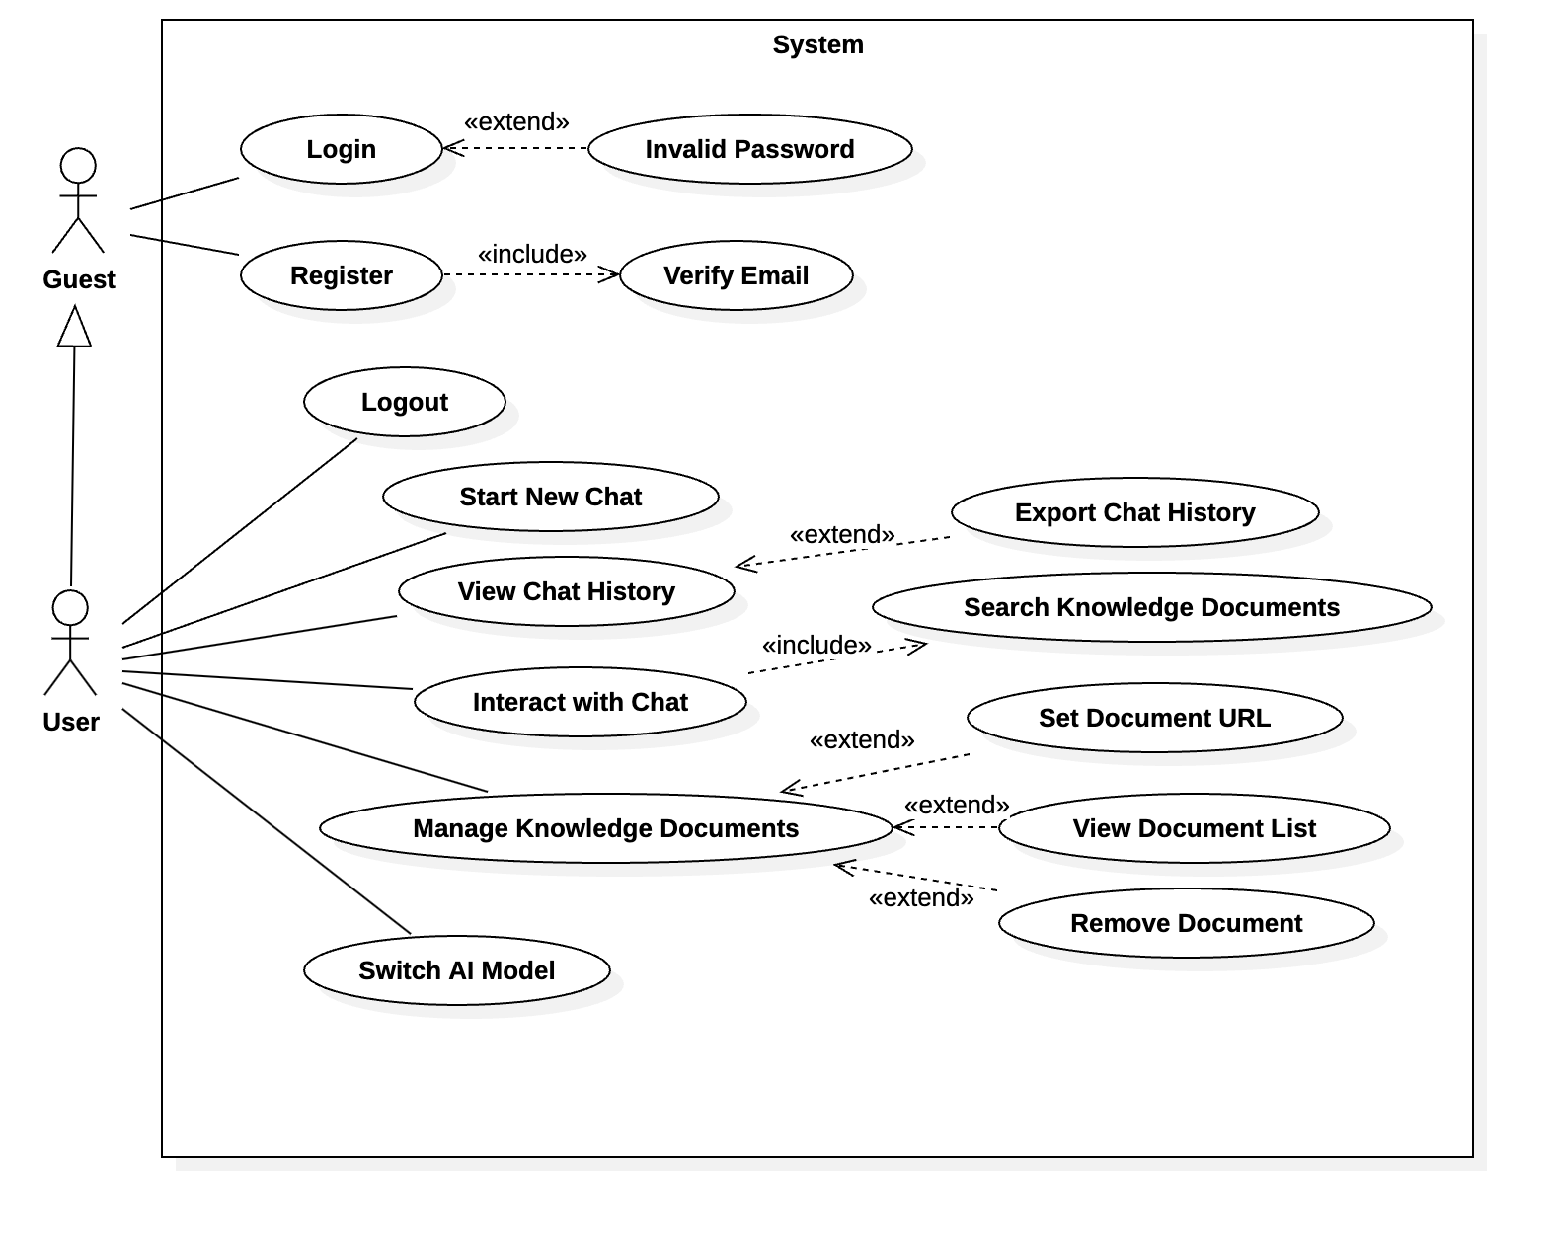
\includegraphics[width=0.8\textwidth]{figures/UseCaseDiagram.pdf}
    \caption{系统用例图} % 添加图片标题
    \label{fig:UseCaseDiagram} % 为图片添加标签,方便在文档中引用
\end{figure}
接下来将介绍其中一些重点用例的用例模型,包括活动图及用例描述表。
根据所属子系统定义用例名称,如表 11 所示。
% 系统用例表
\begin{table}[H] % 表格位置固定
    \centering % 表格整体居中
    \caption{系统用例表} % 表格表题
    \label{tab:system-use-case} % 表格标签
    \renewcommand\arraystretch{0.85} % 定义表格行距
    \setlength{\tabcolsep}{12pt} % 定义列间宽度
    \begin{tabular}{ccc} % 表格列样式定义
        \toprule[1.5pt] % 顶线
        \textbf{所属子系统/功能分类} & \textbf{用例 ID} & \textbf{用例名称} \\ % 表头
        \midrule[0.8pt] % 栏目线
        % 用例
        \multirow{2}{*}{RAG文档检索子系统} & UC-01 & 文档URL精确检索 \\
        & UC-02 & 代码片段检索 \\
        \midrule[0.5pt]
        \multirow{3}{*}{代码生成优化子系统} & UC-03 & 智能代码生成 \\
        & UC-04 & 代码优化建议 \\
        & UC-05 & 性能瓶颈分析 \\
        \midrule[0.5pt]
        \multirow{3}{*}{代码试运行子系统} & UC-06 & 代码试运行 \\
        & UC-07 & 错误检测纠正 \\
        & UC-08 & 调试辅助支持 \\
        \midrule[0.5pt]
        \multirow{2}{*}{模型管理子系统} & UC-09 & 模型切换 \\
        & UC-10 & 自定义模型配置 \\
        \midrule[0.5pt]
        \multirow{4}{*}{用户管理子系统} & UC-11 & 用户注册 \\
        & UC-12 & 用户登录 \\
        & UC-13 & 个人信息管理 \\
        & UC-14 & 个性化偏好设置 \\
        \hline\hline % 底线
    \end{tabular}
\end{table}

\begin{enumerate}[label=(\arabic*)]
    \item 文档URL精确检索
    
    用户通过设置文档URL,并开启文档检索功能,即可实现文档URL精确检索。系统会检查用户设置的文档URL是否符合要求,然后检查文档是否已经存储在系统的向量数据库中。如果文档不存在,系统会提示用户添加文档。如果文档存在,系统会启用QA问答功能,为用户提供文档内容的详细回答。
    如果文档不存在,系统会开始文档添加流程,包括文档内容的提取、向量化存储等。活动图如图 11 所示。
    % \begin{figure}[h] % 创建一个图片环境,[h]表示图片尽量放在当前位置
    %     \centering % 使图片居中
    %     \includegraphics[width=0.8\textwidth]{figures/DocumentAdditionActivityDiagram.pdf}
    %     \caption{文档添加活动图} % 添加图片标题
    %     \label{fig:DocumentAdditionActivityDiagram} % 为图片添加标签,方便在文档中引用
    % \end{figure}
    
    \item 代码片段检索
    
    用户通过设置代码片段,并开启代码检索功能,即可实现代码片段检索。系统会检查用户设置的代码片段是否符合要求,然后读取代码片段内容,并分析代码片段的语义。给出详尽且切实可行的优化方案。系统采用先进的嵌入向量技术,能够理解代码的上下文关系,识别出代码中的模式和结构,从而提供准确的检索结果。
    % \begin{figure}[h]
    %     \centering
    %     \includegraphics[width=0.8\textwidth]{figures/CodeSnippetRetrievalFlow.pdf}
    %     \caption{代码片段检索流程图}
    %     \label{fig:CodeSnippetRetrievalFlow}
    % \end{figure}

    \item 智能代码生成

    用户输入自然语言描述的编程需求或问题,系统利用RAG技术检索相关文档和代码示例,结合大语言模型进行推理,生成符合最新技术规范且准确无误的代码片段。系统支持多种编程语言,包括但不限于Python、JavaScript、Java、C++等,能够根据用户的具体需求,生成各类功能模块的代码实现。生成的代码会自动包含必要的注释和错误处理机制,提高代码可读性和健壮性。
    % \begin{figure}[h]
    %     \centering
    %     \includegraphics[width=0.8\textwidth]{figures/IntelligentCodeGeneration.pdf}
    %     \caption{智能代码生成流程}
    %     \label{fig:IntelligentCodeGeneration}
    % \end{figure}
    
    \item 代码优化建议
    
    系统对用户提交的代码进行多维度分析,包括时间复杂度、空间复杂度、代码风格、设计模式应用等方面,识别可优化的部分,并提供具体的优化建议。系统基于大量真实项目的最佳实践案例库,结合RAG技术检索到的相关优化模式,为用户提供针对性的代码重构和优化策略,帮助用户提升代码质量和运行效率。
    % \begin{figure}[h]
    %     \centering
    %     \includegraphics[width=0.8\textwidth]{figures/CodeOptimizationSuggestions.pdf}
    %     \caption{代码优化建议流程}
    %     \label{fig:CodeOptimizationSuggestions}
    % \end{figure}
    
    \item 性能瓶颈分析
    
    针对用户提交的代码,系统通过静态分析与模拟运行相结合的方式,识别代码中可能存在的性能瓶颈,如算法效率低下、内存泄漏、资源竞争等问题。系统会生成详细的性能分析报告,标注出影响性能的关键代码位置,并提供相应的优化方案。对于复杂系统,还能够进行全局性能评估,协助用户制定系统性能提升策略。
    % \begin{figure}[h]
    %     \centering
    %     \includegraphics[width=0.8\textwidth]{figures/PerformanceBottleneckAnalysis.pdf}
    %     \caption{性能瓶颈分析流程}
    %     \label{fig:PerformanceBottleneckAnalysis}
    % \end{figure}
    
    \item 代码试运行
    
    用户可在系统内输入代码片段,选择目标编程语言及运行环境,点击试运行按钮后,系统会创建一个安全的沙箱环境,迅速执行代码,并将运行结果、控制台输出以及可能出现的错误信息实时反馈给用户。系统支持设置运行参数,如输入值、环境变量等,使用户能够在不同条件下测试代码行为,验证代码逻辑是否符合预期。
    % \begin{figure}[h]
    %     \centering
    %     \includegraphics[width=0.8\textwidth]{figures/CodeTrialRunSystem.pdf}
    %     \caption{代码试运行系统架构}
    %     \label{fig:CodeTrialRunSystem}
    % \end{figure}
    
    \item 错误检测纠正
    
    当代码试运行出现错误时,系统自动启动错误检测与纠正机制。系统会分析错误类型、出错位置及上下文环境,通过与类似错误案例的匹配及RAG技术检索相关解决方案,为用户提供详细的错误解释及修正建议。针对常见错误,系统甚至可以自动生成修复后的代码,用户只需确认即可应用修复。系统还会记录错误及修复方案,不断丰富错误处理知识库。
    % \begin{figure}[h]
    %     \centering
    %     \includegraphics[width=0.8\textwidth]{figures/ErrorDetectionCorrection.pdf}
    %     \caption{错误检测纠正流程}
    %     \label{fig:ErrorDetectionCorrection}
    % \end{figure}
    
    \item 调试辅助支持
    
    系统提供强大的调试辅助功能,帮助用户快速定位和解决代码问题。用户可以设置断点、查看变量状态、执行单步调试等操作,系统会实时显示程序执行流程和数据变化。结合RAG技术,系统能够识别调试过程中的异常状态,并推荐可能的调试策略,如查看特定变量、检查特定函数调用等。系统还支持条件断点和日志点设置,方便用户针对复杂场景进行精细调试。
    % \begin{figure}[h]
    %     \centering
    %     \includegraphics[width=0.8\textwidth]{figures/DebuggingAssistance.pdf}
    %     \caption{调试辅助支持功能示意图}
    %     \label{fig:DebuggingAssistance}
    % \end{figure}
    
    \item 模型切换
    
    用户可在系统界面便捷地切换内置的多个模型,如OpenAI gpt-4o、Qwen-2.5-70B-Instruct等。系统会显示各模型的基本参数、适用场景和性能特点,帮助用户根据具体需求选择最适合的模型。切换模型后,系统会自动调整相关参数设置,以优化所选模型的性能表现。对于高级用户,系统还提供模型参数微调功能,可以根据特定任务对模型行为进行个性化调整。
    % \begin{figure}[h]
    %     \centering
    %     \includegraphics[width=0.8\textwidth]{figures/ModelSwitchingInterface.pdf}
    %     \caption{模型切换界面示意图}
    %     \label{fig:ModelSwitchingInterface}
    % \end{figure}
    
    \item 自定义模型配置
    
    系统支持用户自主调用Hugging Face平台上的其他模型,满足不同用户对模型性能、风格和专业性的多样化需求。用户可以指定模型名称、版本,并配置相关参数,如温度系数、采样方式、最大输出长度等。系统会处理API调用、模型加载和资源分配,确保自定义模型能够高效稳定地运行。对于专业用户,系统还支持模型微调和参数优化,以适应特定领域的任务需求。
    % \begin{figure}[h]
    %     \centering
    %     \includegraphics[width=0.8\textwidth]{figures/CustomModelConfiguration.pdf}
    %     \caption{自定义模型配置流程}
    %     \label{fig:CustomModelConfiguration}
    % \end{figure}
    
    \item 用户注册
    
    用户通过填写基本信息(如用户名、邮箱)并设置密码来创建账号。系统会验证用户提供的信息有效性,检查用户名是否已被占用,邮箱是否合法等。注册成功后,系统会发送验证邮件,用户完成验证后即可激活账号。
    % \begin{figure}[h]
    %     \centering
    %     \includegraphics[width=0.8\textwidth]{figures/UserRegistrationFlow.pdf}
    %     \caption{用户注册流程}
    %     \label{fig:UserRegistrationFlow}
    % \end{figure}
    
    \item 用户登录
    
    用户通过输入注册时使用的账号(邮箱)和密码进行身份验证,系统验证信息无误后允许用户访问个人账号。系统支持记住登录状态功能,用户可选择在特定设备上保持登录状态,免去频繁登录的麻烦。对于安全敏感的操作,系统会要求用户进行二次验证,如输入验证码、回答安全问题等。
    % \begin{figure}[h]
    %     \centering
    %     \includegraphics[width=0.8\textwidth]{figures/UserLoginProcess.pdf}
    %     \caption{用户登录流程}
    %     \label{fig:UserLoginProcess}
    % \end{figure}
    
    \item 个人信息管理
    
    用户可在个人中心查看、修改自己的基本信息,包括昵称、密码、邮箱等。系统提供个人资料完整度提示,鼓励用户完善信息以获得更好的服务体验。用户可以管理自己的账号安全设置,如修改密码、绑定邮箱等。% 系统还支持查看账号活动历史,包括登录记录、操作日志等,帮助用户监控账号安全状态,及时发现异常情况。
    % \begin{figure}[h]
    %     \centering
    %     \includegraphics[width=0.8\textwidth]{figures/PersonalInfoManagement.pdf}
    %     \caption{个人信息管理界面}
    %     \label{fig:PersonalInfoManagement}
    % \end{figure}
    
    \item 个性化偏好设置
    
    用户可根据自身习惯和需求,定制系统的各项参数和功能展示。可设置的偏好包括界面主题(明亮/暗黑模式)、代码编辑器风格、默认编程语言、常用代码模板等。用户还可以调整系统的交互方式,如是否自动运行代码、是否显示详细错误信息、代码提示的触发方式等。系统会记住这些设置并在用户每次登录时自动应用,同时支持设置导出与导入,方便用户在多设备间同步偏好配置。
    % \begin{figure}[h]
    %     \centering
    %     \includegraphics[width=0.8\textwidth]{figures/PersonalizedPreferences.pdf}
    %     \caption{个性化偏好设置页面}
    %     \label{fig:PersonalizedPreferences}
    % \end{figure}
\end{enumerate}

\subsection{软件需求的用例交互模型}

用例交互模型描述了用户与系统之间的交互过程,包括用户的操作请求和系统的响应行为。下面详细说明主要用例的交互模型。

\begin{enumerate}[label=(\arabic*)]
    \item 文档URL精确检索交互模型
    
    文档URL精确检索的交互流程始于用户在系统界面输入文档URL,系统接收并验证URL有效性。若URL有效,系统查询向量数据库确认该文档是否已存储。对于已存储的文档,系统直接呈现与文档相关的交互界面,允许用户输入问题进行精确查询;系统内部会调用RAG引擎,将用户问题与文档内容进行语义匹配,返回最相关的回答。
    
    若文档未存储,系统弹出确认对话框,征求用户是否添加该文档。用户确认后,系统启动文档爬取与处理模块,解析网页内容、提取文本、分割文档并进行向量化处理,最终存入向量数据库。处理完成后,系统通知用户,并转入问答交互界面。整个交互过程以图形界面提示和进度反馈为主,确保用户了解当前操作状态。
    % \begin{figure}[h]
    %     \centering
    %     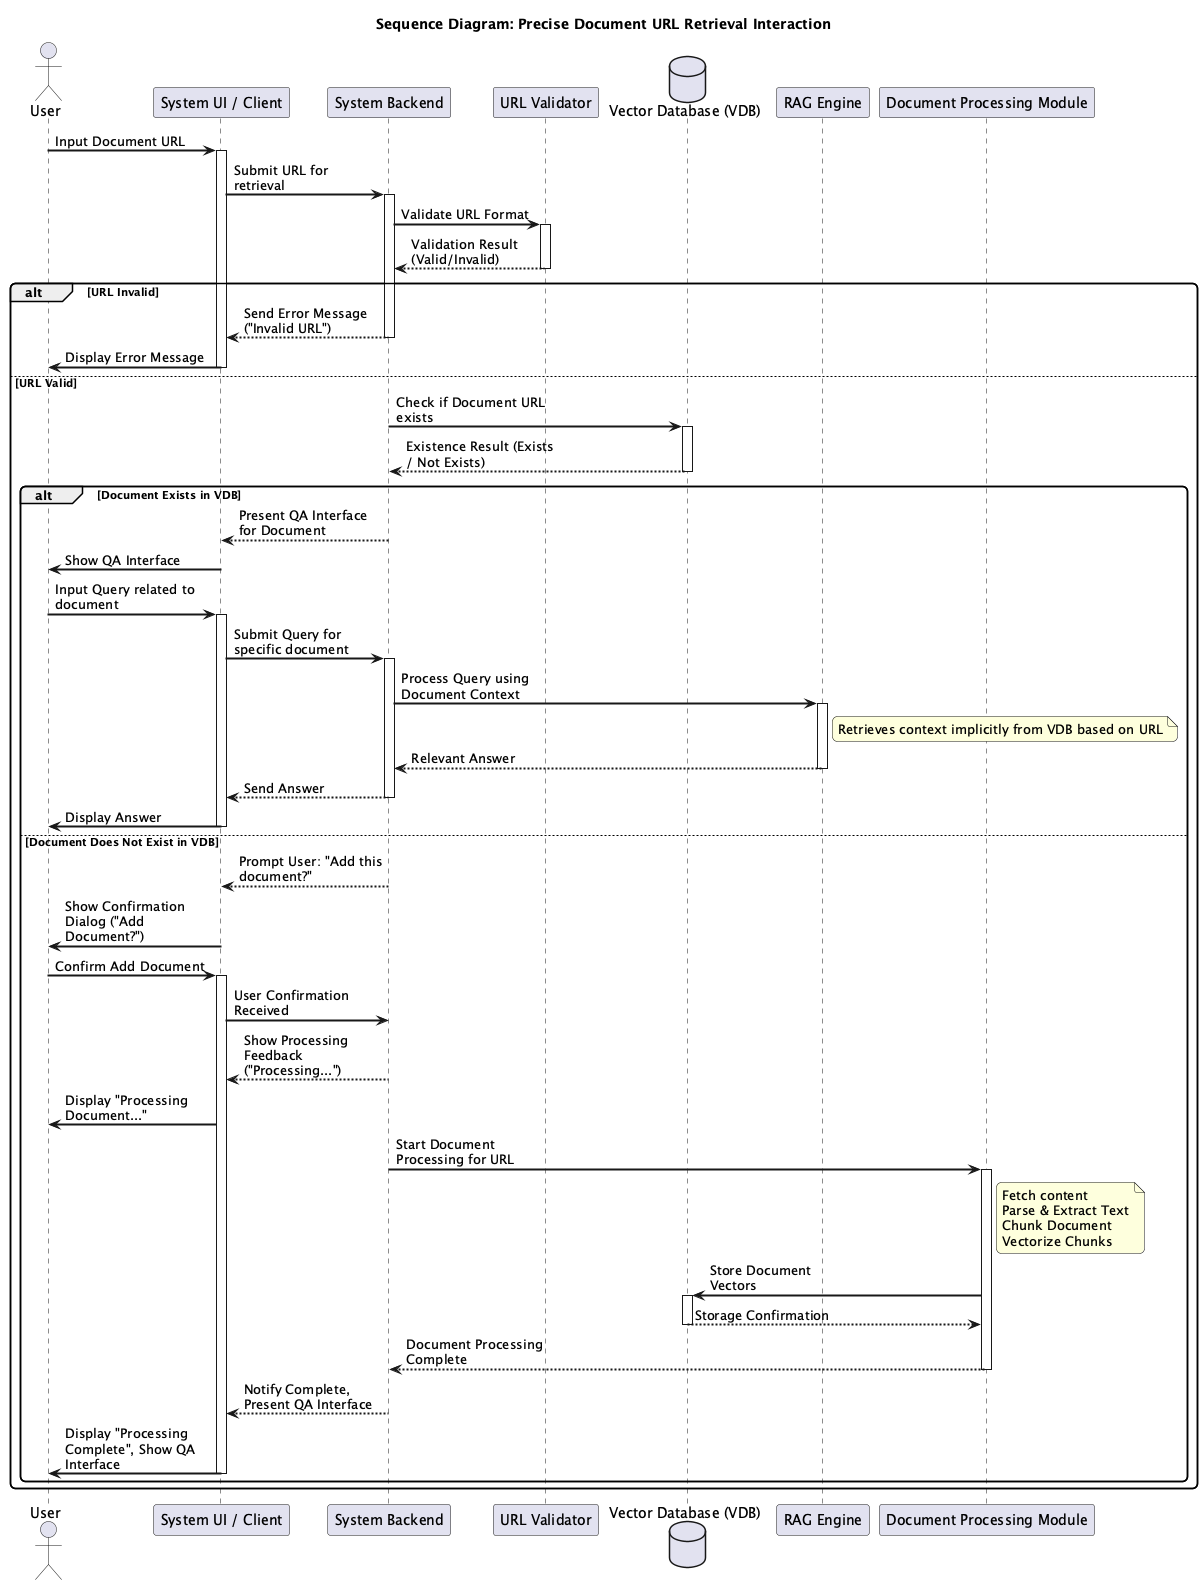
\includegraphics[width=0.8\textwidth]{figures/DocumentRetrievalSequenceDiagram.pdf}
    %     \caption{文档URL精确检索时序图}
    %     \label{fig:DocumentRetrievalSequenceDiagram}
    % \end{figure}
    
    \item 代码生成交互模型
    
    智能代码生成交互流程开始于用户在编辑器中输入自然语言描述的编程需求。用户可以指定目标编程语言、框架及其他相关参数,然后触发代码生成请求。系统接收请求后,会将用户需求传递给RAG处理模块,该模块首先检索相关技术文档和代码案例,提取有价值的参考信息。
    
    接着,系统将检索结果与用户需求一同传递给大模型推理引擎,由其生成初步代码。系统对生成的代码进行静态分析和语法检查,确保其符合目标语言规范且无明显错误。最终,系统将优化后的代码返回给用户界面,以编辑器友好的格式呈现,包括语法高亮、代码缩进等。用户可以直接编辑生成的代码,或请求系统解释特定代码段,或要求系统基于反馈进行代码调整。
    % \begin{figure}[h]
    %     \centering
    %     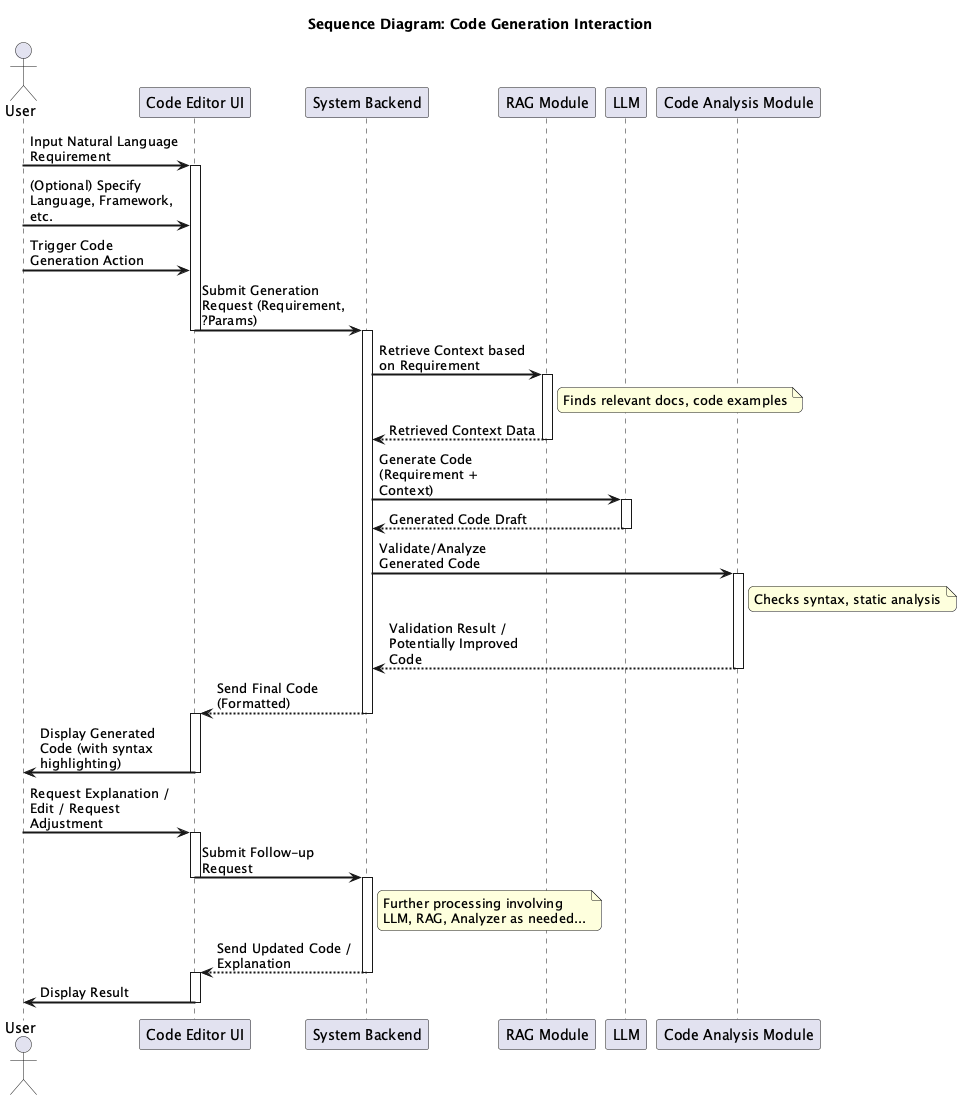
\includegraphics[width=0.8\textwidth]{figures/CodeGenerationSequenceDiagram.pdf}
    %     \caption{智能代码生成时序图}
    %     \label{fig:CodeGenerationSequenceDiagram}
    % \end{figure}
    
    \item 代码试运行交互模型
    
    代码试运行的交互始于用户在代码编辑区输入或修改代码后,选择目标运行环境和语言版本,然后点击"运行"按钮。系统首先验证代码格式是否符合所选语言的基本语法规范,如有明显语法错误,会立即反馈给用户。
    
    验证通过后,系统创建隔离的沙箱环境,配置必要的运行时依赖,并将代码注入环境中执行。执行过程中,系统实时捕获标准输出、错误输出和运行状态,在界面上显示执行进度。当代码运行完成或遇到错误时,系统收集所有输出信息和错误堆栈,格式化后呈现给用户。
    
    若执行过程中出现错误,系统自动启动错误分析模块,识别错误类型并提供修复建议。对于常见错误模式,系统可直接提供修复后的代码示例。用户可查看详细的运行日志,并基于系统建议修改代码再次尝试运行,形成迭代优化的交互循环。
    % \begin{figure}[h]
    %     \centering
    %     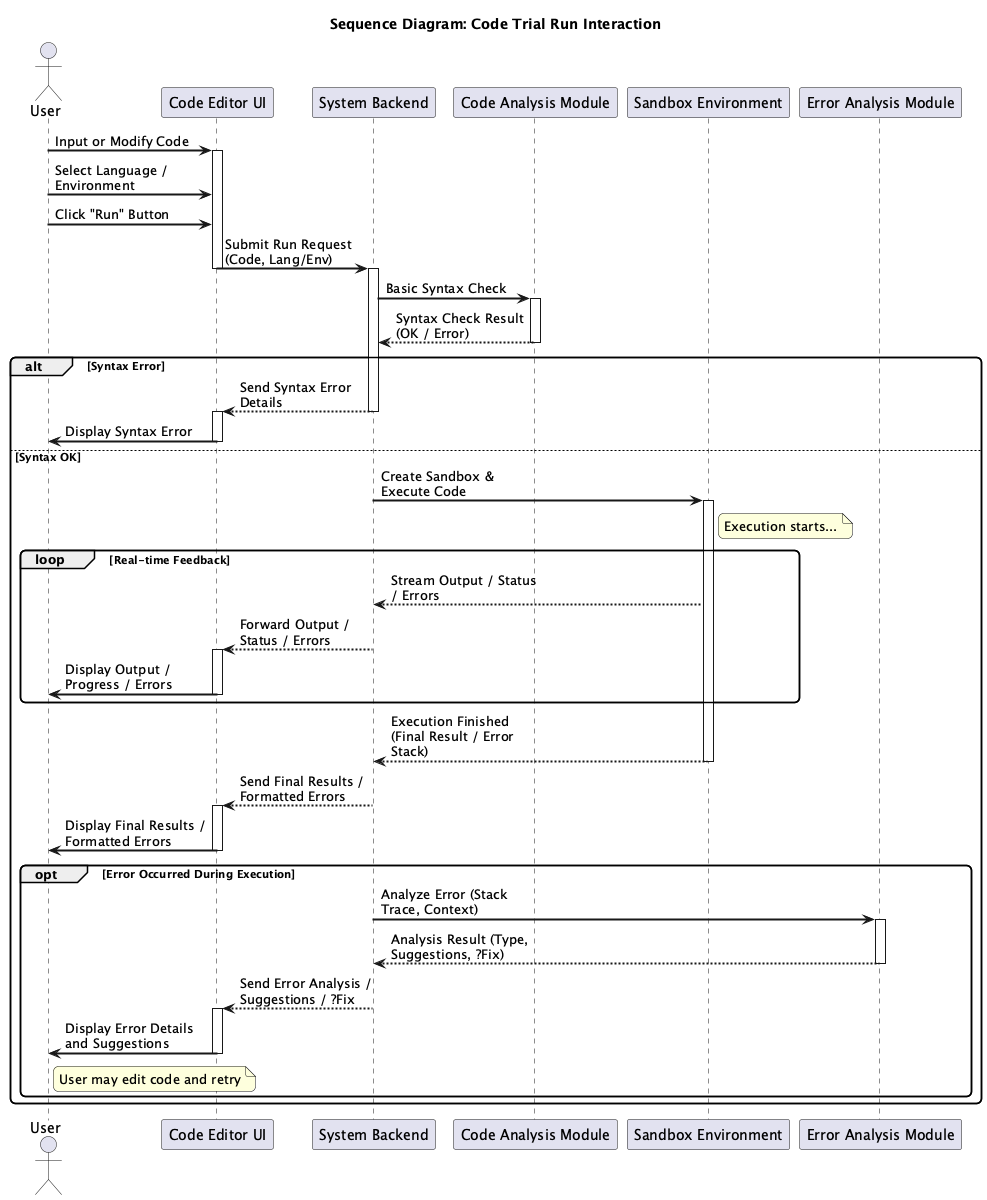
\includegraphics[width=0.8\textwidth]{figures/CodeRunSequenceDiagram.pdf}
    %     \caption{代码试运行时序图}
    %     \label{fig:CodeRunSequenceDiagram}
    % \end{figure}
    
    \item 模型切换交互模型
    
    模型切换交互流程始于用户点击系统界面上的模型选择区域,系统随即展示当前可用的AI模型列表,包括每个模型的基本信息(名称、版本)、特性说明和适用场景。用户从列表中选择目标模型后,系统后台启动模型资源调度流程。
    
    系统首先检查选定模型的资源状态,判断是否需要加载或初始化。对于已加载的模型,系统直接切换API调用目标;对于未加载的模型,系统先释放当前模型占用资源,然后加载新模型到内存。加载过程中,界面显示加载进度条,并提示用户稍候。
    
    模型切换完成后,系统自动调整配置参数以优化所选模型的表现,并更新界面状态指示当前激活的模型。用户可以在模型详情面板查看和调整各项参数,如推理温度、最大输出长度等,系统即时应用这些设置,并在下一次交互中生效。
    % \begin{figure}[h]
    %     \centering
    %     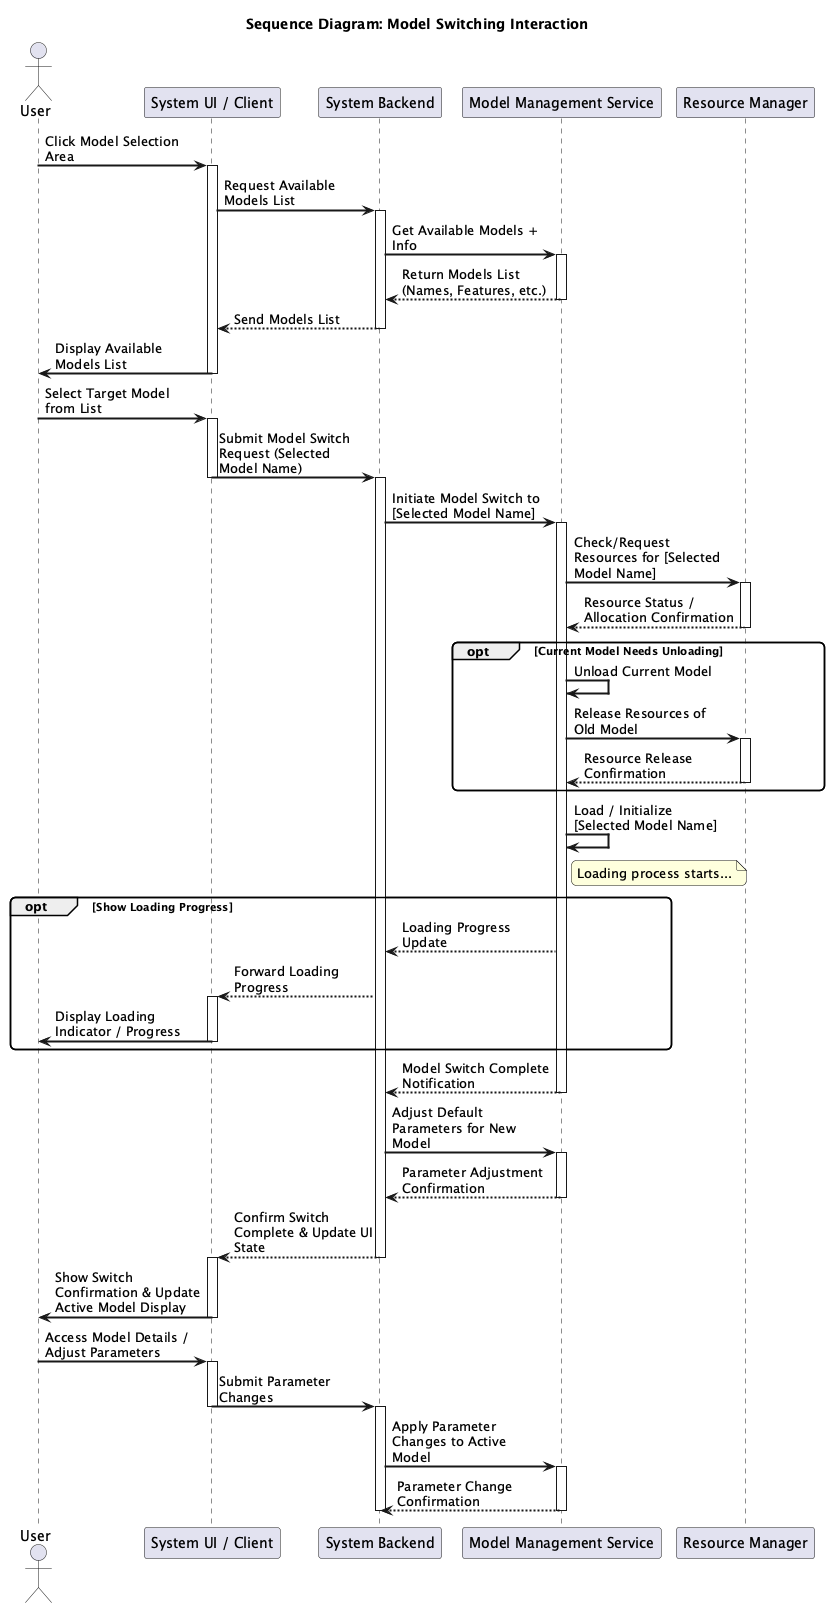
\includegraphics[width=0.8\textwidth]{figures/ModelSwitchingSequenceDiagram.pdf}
    %     \caption{模型切换时序图}
    %     \label{fig:ModelSwitchingSequenceDiagram}
    % \end{figure}
    
    \item 用户注册与登录交互模型
    
    用户注册交互始于用户访问注册页面并填写必要的个人信息(用户名、邮箱、密码等)。提交表单后,系统进行表单验证,检查信息是否完整、邮箱格式是否正确、用户名是否已被占用等。验证通过后,系统创建用户记录,生成随机验证码,并向用户提供的邮箱发送验证邮件。
    
    用户通过邮件中的验证链接或直接输入验证码完成邮箱验证。验证成功后,系统激活用户账号,并自动将用户重定向到登录页面或直接登录到系统首页,同时展示欢迎消息和基本使用指引。
    
    用户登录交互则从登录页面开始,用户输入邮箱和密码后,系统验证凭据的有效性。验证通过后,系统生成授权令牌,设置会话状态,并将用户重定向到系统主界面。如用户开启了记住登录选项,系统会设置持久化的登录凭证,使用户在下次访问时无需重新登录。整个过程中,系统提供清晰的状态反馈,确保用户了解每一步的结果。
    % \begin{figure}[h]
    %     \centering
    %     \includegraphics[width=0.8\textwidth]{figures/UserAuthSequenceDiagram.pdf}
    %     \caption{用户注册与登录时序图}
    %     \label{fig:UserAuthSequenceDiagram}
    % \end{figure}
\end{enumerate}

\subsection{软件需求的分析类模型}

在分析了用例模型与用例交互模型后,我们构建了初步的分析类模型,明确了类之间的关系和属性,并绘制了相应的类图,如图18 所示。
% \begin{figure}[H]
%     \centering
%     \includegraphics[width=0.8\textwidth]{figures/analysis-class-model.pdf}
%     \caption{软件需求的分析类模型}
%     \label{fig:analysis-class-model}
% \end{figure}

\section{其它软件需求描述}
\subsection{性能要求}
\begin{enumerate}[label=(\arabic*)]
    \item 所有界面操作的响应时间应小于1 秒
    \item 内存占用率应小于等于 50%
    \item 数据的转换和传送时间应小于 2 秒
    \item 系统应能支持至少100 个并发用户同时操作,而不影响性能或稳定性
    \item 系统应每周七天,每天24 小时可用;在没有故障的情况下系统正常运行时间比例在95\%以上
    \item 系统任何故障都不应导致用户已提交数据的丢失,发生故障后,系统应能在 10分钟内恢复到正常运行状态
\end{enumerate}

\subsection{设计约束}

\begin{enumerate}[label=(\arabic*)]
    \item 开发工具:使用Python作为主要开发语言,采用FastAPI框架进行开发,确保系统的可维护性和可扩展性。
    \item 运行环境:使用RockyLinux 9.5作为运行环境,确保系统的稳定性和安全性。
    \item 安全性需求:系统应具备基本的安全防护措施,包括但不限于数据加密、身份验证、访问控制等。
\end{enumerate}
\subsection{界面要求}
\begin{enumerate}[label=(\arabic*)]
    \item 直观性:界面设计应简洁明了,避免过多的冗余元素,使用户能够迅速找到所需
    功能。
    \item 易用性:提供清晰的导航菜单,帮助用户了解当前所在位置和快速跳转至其他页
    面。
    \item 美观性:采用合适的配色方案,使界面看起来舒适、美观,并符合旅游行业的风
    格。
\end{enumerate}
\subsection{进度要求}
最迟在2025年6月3日前完成开发
\subsection{交付要求}
\begin{enumerate}[label=(\arabic*)]
    \item 交付内容:各阶段形成的报告、完整的可执行系统。
    \item 交付形式:所有内容以电子文件形式交付。
\end{enumerate}
\subsection{验收要求}
\begin{enumerate}[label=(\arabic*)]
    \item 功能性要求:验证产品是否满足所有预定的功能需求,包括但不限于用户界面、代码生成、代码优化、代码调试、代码文档生成等功能。
    \item 性能要求:系统的响应速度、处理能力、并发用户数等性能指标是否达到预期要求。
    \item 安全性要求:系统是否采取了必要的安全措施,如用户认证、权限管理、数据加
    密等。
\end{enumerate}
\section{软件原型}
项目采用figma进行界面原型设计
\chapter{软件设计规格说明书}
\section{引言}
\subsection{编写目的}
\subsection{读者对象}
\subsection{软件项目概述}
\subsection{文档概述}
\subsection{定义}
\subsection{参考资料}
\section{软件设计约束}
\subsection{软件设计目标和原则}
\subsection{软件设计的约束和限制}
\section{软件设计}
\subsection{软件体系结构设计}
\subsection{用户界面设计}
\subsection{用例设计}
\subsection{数据设计}
\chapter{软件测试计划书}
\section{引言}
\subsection{编写目的}
\subsection{背景}
\subsection{定义}
\subsection{参考资料}
\section{单元测试}
\subsection{测试目的}
\subsection{测试内容}
\section{集成测试}
\subsection{测试目的}
\subsection{测试内容}
\section{确认测试}
\subsection{测试1}
\subsection{测试2}
\subsection{测试3}
\subsection{测试4}
\subsection{测试5}
\subsection{测试6}

\section{评价准则}
\subsection{范围}
\subsection{数据整理}
\subsection{尺度}
\chapter{总结}


%%%%%%%%%%%%%%%%%%%%%%%%  参考文献  %%%%%%%%%%%%%%%%%%%%%%%%

%\begin{references}
%    \bibliography{references.bib} % 指定.bib文件路径
%\end{references}

%%%%%%%%%%%%%%%%%%%%%%%%%  附录  %%%%%%%%%%%%%%%%%%%%%%%%%%

%\StartAppendix % 启用附录

%\chapter{附录}

%附录

%%%%%%%%%%%%%%%%%%%%%%%  正文后页眉  %%%%%%%%%%%%%%%%%%%%%%

% 页眉(关闭页眉务必将页眉类型设为empty)
\Header
    {common} % 页眉类型:common、publish、empty
    {1pt} % 上分隔线宽度
    {1pt} % 两线距离
    {0.5pt} % 下分割线宽度
    {} % 页眉左自定义内容(文本或图片)
    {
\includegraphics[width=0.25\textwidth]{figures/logos/SXU-title-EN.png}} % 页眉中自定义内容(文本或图片)
    {} % 页眉右自定义内容(文本或图片)

%============================================%

% 页脚(关闭页脚务必将页脚类型设为empty) 
\Footer
    {common} % 页脚类型:common、publish、empty
    {0pt} % 上分隔线宽度
    {0pt} % 两线距离
    {0pt} % 下分割线宽度
    {} % 页脚左自定义内容(文本或图片)
    {\thepage} % 页脚中自定义内容(文本或图片)
    {} % 页脚右自定义内容(文本或图片)

%============================================%

% 页数样式 参数:#1起始页数
% \setRomanPageNumber{1} % 设置罗马数字页码
% \setArabicPageNumber{1} % 设置阿拉伯数字页码

%%%%%%%%%%%%%%%%%%%%%%%%%  致谢  %%%%%%%%%%%%%%%%%%%%%%%%%

%\StartAcknowledgements % 启用致谢

%致谢

\end{document}